\documentclass[12pt]{article}
\title{Samenvatting Bedrijfskunde [H01F2A]}
\author{Wouter Schaekers\\*---\\*Bachelor Ingenieurswetenschappen\\*Master Ingenieurswetenschappen: Computerwetenschappen}
\date{January, 2014}
\usepackage{amsmath}
\usepackage[top=25mm, bottom=25mm, left=25mm, right=25mm]{geometry}
\usepackage[colorlinks = true,
            linkcolor = blue,
            urlcolor  = blue,
            citecolor = blue,
            anchorcolor = blue]{hyperref}
\usepackage{graphicx}
\usepackage[toc,page]{appendix}
\usepackage{pdfpages}
\usepackage{fancyhdr}
\begin{document}
\pagestyle{fancy}
\maketitle
\setcounter{page}{0}
\setcounter{section}{-1}
\renewcommand{\contentsname}{Inhoudstafel}
\setcounter{tocdepth}{3}
\tableofcontents
\clearpage
\section{Inleiding}
Deze samenvatting is opgesteld aan de hand van de twee boekjes van Ludo Gelders, Beginselen van de Bedrijfskunde en Technische Bedrijfsvoering en Organisatie. Voor beide boekjes heb ik de 5de en 4de druk gebruikt (2012). In deze samenvatting zullen vaak verwijzingen staan naar prentjes in het tekstboek. Indien u een andere druk gebruikt dan diegene die ik hanteer, kan het zijn dat de paginanummers niet overeen komen. In dat geval hebt u pech.\\*
Aangezien cursusen tegenwoordig slechts 5\% bevatten en voor de rest gezever, heb ik de totaal aantal paginas sterk kunnen reduceren. Deze samenvatting is opgesteld met het idee dat dit vak succesvol kan worden afgelegd, enkel en alleen aan de hand van deze samenvatting. Hiermee beweer ik niet dat deze samenvatting volledig is. Integendeel. De hoofdstukken 6 en 7 van de Engelstalige teksten heb ik niet samengevat, wegens veel te veel tekst voor veel te weinig inhoud (en te weinig tijd). Het is mogelijk dat deze samenvatting zal worden vervolledigd indien ik hier meer tijd voor kan vinden. Alle andere onderdelen zijn wel volledig behandeld. Vergeet niet dat niet alle hoofdstukken gekend moeten zijn, ook al zijn deze samengevat. Maak dus niet dezelfde fout als ik gemaakt heb!\\*
Indien je lege secties tegenkomt, is dit niet omdat ik deze vergeten ben, maar omdat deze secties veel gemekker bevatten zonder inhoud.
Dit is enkel een samenvatting van de cursustekst, niet van de bijbehorende slides.\\*
Deze samenvatting is hoogstwaarschijnlijk niet foutloos. Eventuele aanpassingen kunnen gemaakt worden op https://github.com/WouterSchaekers/Bedrijfskunde-Samenvatting.\\*
Appendix \ref{sec:Begrippen} bevat een lijst met begrippen die opgesteld is door een andere student. Deze lijst ziet er vrij volledig uit. Het heeft geen zin om dubbel werk te verrichten.
\clearpage
\noindent De auteur is niet bereid samenvattingen te signeren.\\*
Het sturen van spam is verboden. Het stalken van de auteur is, na toestemming, slechts in uitzonderlijke omstandigheden toegestaan.\\*
De auteur is niet verantwoordelijk voor enige gevolgen van het gebruik van deze bundel. Indien u zich beledigd voelt door de inhoud van deze samenvatting, gelieve te stoppen met het lezen van deze samenvatting en uzelf terug te trekken in uw bunker.\\*
Het is verboden de afgedrukte versie van de samenvatting te verbranden of op te eten.\\*\\*
Geen langdurig gebruik zonder wiskundig advies.\\*\\*
Alle lijnstukken voorbehouden. Niet op de openbare weg gooien.\\\\
This resume is released under the beerware license. Donations on the following bitcoin address are really appreciated. Thanks.\\\\\\\\\\\\\\\\\\\\\\\\\\\\\\\\\\\\\\
\begin{center}
\textit{"Alles moet zo eenvoudig mogelijk gemaakt worden, maar niet eenvoudiger dan dat."}\\*-\\*Albert Einstein
\end{center}
\begin{center}

\includegraphics[scale=0.5]{BitcoinAddress.png}\\*

\includegraphics[scale=0.02]{Bitcoin.png} \textbf{1CCDinUvtZXtqSsrHLQxtfV2YLu9WHR72f}
\end{center}
\clearpage
\section{Hoofdstuk 1: Inleiding}
\subsection{Beleid en ondernemerschap}
4M's: Men-Materials-Money-Management.\\*
Duurzaam ondernemen: De onderneming is een schakel in een complex geheel. De onderneming moet rekening houden met het welzijn van alle stakeholders (werknemers, consumenten, de overheid, ...) en niet enkel de stockholders (eigenaars).
\subsection{Duurzame ontwikkeling en duurzaam ondernemen}
\subsection{Maatschappelijke context en finaliteit van de onderneming}
Meerwaarde ($MW$) = Inkomsten ($I$) - Uitgaven ($U$) = Vergoeding lonen ($V_L$) + Vergoeding voor de gemeenschap ($V_G$) + Vergoeding voor het kapitaal ($V_K$) + Autofinanciering ($AF$)
\subsection{Organisatie en beheer}
\subsection{Innovatie en onderneming}
Innovatie doet zich voor op verschillende manieren:
\begin{itemize}
\item Productieverhoging/Kostenverlaging.
\item Innovatie van de producten zelf $\rightarrow$ differenti\"ering.
\item Innovatie van de arbeidsorganisatie.
\item De verkorting van de doorlooptijd en de juiste keuze van het moment waarop een product op de markt wordt gebracht.
\end{itemize}
Voor de rest staat er een hoop geblaat in dit hoofdstuk (een heel deel komt later terug, dus het heeft geen zin deze zaken hier te vermelden). Het is dan ook de inleiding.
\clearpage
\section{Hoofdstuk 2: Productlevenscyclus}
\subsection{Begrip 'productlevenscylcus'}
De productlevenscyclus bestaat uit vijf stadia: de introductie, de vroege groei, de late groei, de maturiteit en tot slot het verval.
Voor de introductie gaat er nog een fase aan vooraf, de embryonale fase. Hier wordt het idee ontwikkeld. Zowel tijdens de embryonale fase als tijdens de introductie is de eenheidswinst negatief, wat wil zeggen dat het bedrijf verlies maakt. Dit brengt een \textit{consumentenrisico} met zich mee.\\*
Figuur 2.1, blz 26 geeft een samengevatte vergelijking weer tussen de verschillende stadia.\\*
In de pagina's erna wordt elk onderdeel van de PLC besproken. Dit is leuk om te lezen, maar bevat geen informatie.
\subsection{Bedenkingen - Voorbeelden}
\subsubsection{Productcategorie-productsubcategorie-merk-model}
Het woord 'product' kan op verschillende niveaus van aggregatie slaan. Op het hoogste niveau is dit de productcategorie (auto's). Een niveau lager is dit de productsubcategorie (personenwagens). Het woord 'product' kan ook slaan op een merk (Jaguar). Een niveau lager is dit een specifiek model (Golf Diesel).\\*
Het concept PLC is enkel bruikbaar op het niveau van de product(sub)categorie.
\subsubsection{Industrietak - Innovator}
Zie figuur 2.3, blz 31 voor een voorbeeld van hoe een innovator de markt be\"invloedt.
\subsubsection{Verlenging van de PLC}
Soms kan de maturiteit van een product uitgesteld worden:
\begin{itemize}
\item Promotieacties en voordelen
\item Een meer gevarieerd gebruik (nieuwe toepassingen)
\item Het aanspreken van een nieuwe gebruikersgroep
\end{itemize}
Zie figuur 2.4, blz 32 hoe de PLC er uitziet.
\subsubsection{'Foothill'-verschijnsel}
Zie figuur 2.5, blz 33 voor het 'foothill' verschijnsel.\\*
De eerste stijging is te wijten aan testaankopen van de consumenten. Daarna vormen de verbruikers zich een opinie over het product in kwestie (vandaar de daling). Daarna hervat de PLC zich.
\subsubsection{Rageproducten}
Rageproducten kennen geen maturiteitsfase. Zie figuur 2.6, blz 23 voor de PLC.
\subsubsection{Grondstoffen en energie\"en}
De levenscyclus van grondstoffen en energie\"en is afhankelijk van de producten die hieruit vervaardigd worden. Deze hebben dan ook een langdurige maturiteit.
\subsection{Nut van het concept PLC}
Obvious.
\subsection{PLC en kostprijs}
De kostenspecificatie kan even belangrijk zijn als de technische specificatie.\\*
De kosten, opgedeeld in deelkosten voor de verschillende componenten, die uit het proces te voorschijn komen, vormen voor iedereen een doelstelling om na te streven en te verbeteren. (\textit{target costing})
\clearpage
\section{Hoofdstuk 3: Algemene boekhouding}
\subsection{Inleiding}
De onderneming heeft productiemiddelen nodig. Dit zijn externe middelen (grondstoffen, diensten in onderaanneming, \dots) of interne middelen (arbeid, gebouwen, \dots).\\*
De algemene boekhouding is een weerspiegeling van het ondernemingsgebeuren. Op regelmatige tijdstippen zal een balans worden opgemaakt, waarin de opbrengsten met de kosten zullen worden vergeleken.
\subsection{Principes van de algemene boekhouding}
\subsubsection{Begrip}
\subsubsection{De zaaktheorie}
De zaaktheorie maakt een onderscheid tussen het vermogen van de onderneming en het vermogen van de eigenaar(s) van de onderneming. De boekhouding van een onderneming geeft dus een beeld vanuit de onderneming zelf. De eigenaar of de aandeelhouder is dus een buitenstaander. De onderneming heeft ten opzichte van de eigenaar een kapitaalschuld ($S_e$).
\subsubsection{De dubbele boekhouding}
Naast $S_e$ is er ook $S_d$, de schulden ten opzichte van derden.\\*
Alles wat de onderneming bezit zijn de \textit{Bezittingen en Vorderingen} (B). Het is evident dat $B = S_d + S_e$. Er kunnen een aantal zaken gebeuren die de waarden van $B$, $S_d$ of $S_e$ veranderen. Wat er ook gebeurt, de eerder genoemde verhouding blijft steeds geldig.\\*
Er kunnen twee soorten transacties plaatsgrijpen: Innderlijke waardeverschuiving (de verandering gebeurt binnen $B$, $S_d$ of $S_e$ zelf) of waarde-omzetting (de verandering gebeurt tussen $B$, $S_d$ en $S_e$).
\subsection{De balans}
\subsubsection{Begrip}
De balans geeft de toestand van een onderneming weer op een bepaald ogenblik. De balans is in twee delen verdeeld. Het rechtse gedeelte wordt passief genoemd en omvat de bronnen of de schulden van de onderneming. Het linkse gedeelte wordt actief genoemd en omvat het gebruik van deze bronnen (dus de bezittingen). De balans is steeds in evenwicht.
\subsubsection{Inhoud}
Het activa-gedeelte wordt normaal gerangschikt volgens liquiditeitsgraad, met name hoe snel een bestanddeel snel in geld kan worden omgezet. Vaste activa zijn het minst liquide (en staan dus bovenaan in de activa-tabel). Dit zijn bijvoorbeeld het bedrijfsgebouw of de machines die gebruikt worden. Daarnaast zijn er nog de \textit{beschikbare waarden} zoals de Kas, Bank en Postrekening. Tussen deze twee in bevinden zich de \textit{realiseerbare of omzetbare middelen} zoals de Voorraden.\\
De passiva zijn gerangschikt volgens eisbaarheidsgraad (door de externe partij). Het \textit{eigen vermogen} is niet-eisbaar en staat bovenaan. \textit{Schulden op lange en middellange termijn} (minstens \'e\'en jaar) en \textit{Schulden op korte termijn} staan hieronder. Zie figuur 3.3, blz 43 voor een overzicht.
\subsubsection{Belang}
Obvious.\\*
Zie blz 44, onder de tabel voor een voorbeeld van hoe een balans te lezen.
\subsubsection{Wettelijke voorschriften betrefende de verslaggeving}
De \textit{balanswaarheid}: De balans moet een waarheidsgetrouw beeld geven van de onderneming.\\*
De \textit{balanseenheid}: Opeenvolgende balansen moeten \'e\'envormig zijn. Dit wil zeggen dat een vergelijk van opeenvolgende balansen mogelijk moet zijn.\\*
De \textit{balansklaarheid}: Een eenduidige en materi\"ele presentatie van de balans. (Geen flauw idee wat dit wil zeggen.)\\
Nog een aantal zaken waarmee rekening moet worden gehouden:
\begin{itemize}
\item Bij het noteren van de activa moet er rekening gehouden worden met afschrijvingen en waardeverminderingen. De waarde van een product vermindert indien het in gebruik is (bijvoorbeeld door slijtage). Meestal gebeurt dit jaarlijks. Later hierover meer.
\item Overlopende rekeningen zorgen ervoor dat kosten en opbrengsten worden toegerekend aan de periode waarin ze worden gemaakt of verworven. (De balans kan dus voorlopen op de realiteit.)
\item Door inflatie of door een te hoog afschrijvingsritme kunnen bepaalde vaste activa een te lage nettowaarde hebben. Deze moeten geherwaardeerd worden (in de rubriek \textit{Herwaarderingsmeerwaarden}).
\item Het omgekeerde kan ook waar zijn. Mogelijke onverwachte verliezen moeten kunnen ingeschreven worden. Dit gebeurt in de rubriek \textit{Voorzieningen voor verliezen en kosten}.
\end{itemize}
Het is mogelijk om tijdelijk vals te spelen door bepaalde balansposten over (\textit{geflatteerde balans/window dressing}) of onder (\textit{gedeflatteerde/gedeprecieerde}) \textit{balans} te waarderen.
\subsubsection{De sociale balans}
De sociale balans wil, naast het technisch-economische van het bedrijfsgebeuren ook het sociaal-teschnische van dat gebeuren binnen het bereik en de uitdrukkingswijze van de 'balans' brengen. (Personeelsbestand, opleiding, overuren, \dots) Dit valt onder de rubriek \textit{sociale informatie}.
\subsubsection{Boekhouden met opeenvolgende balansen}
Voor elke verrichting kan een nieuwe balans opgesteld worden. Dit is uiteraard omslachtig, tijdrovend en weinig overzichtelijk.
\subsection{De rekening en het journaal}
\subsubsection{De rekening}
In plaats van wijzigingen rechtstreeks in de balans door te voeren, wordt voor elk onderdeel een aparte staat opgemaakt en systematisch aangevuld.\\*
In plaats van alle vermeerderingen en verminderingen door elkaar te mengen in \'e\'en kolom, worden toenamen en afnamen gegroepeerd op de linker- en rechterzijde van de rekening. Een rekening wordt afgesloten door het saldo in te schrijven op de zwakste zijde.\\*
De volledige verzameling gehanteerde rekeningen in een bepaalde onderneming vormt het grootboek.\\*
Sommige van deze rekeningen zijn onderdeel van de balans. Toenamen in activa worden genoteerd aan de debetzijde, afnamen aan de creditzijde. Voor passiva is dit omgekeerd. Leuk ezelsbruggetje: Credit is Cashen, Debet is Dokken!\\*
De andere rekeningen komen in de resultatenrekeningen. Ook hier wordt hetzelfde onderscheid gemaakt onder de vorm van een Kostenrekening en een Opbrengstenrekening.\\*
Alle rekeningen worden uiteindelijk in het dagboek of journaal in een chronologische volgorde genoteerd.\\*
Vaak zal men een boel transacties groeperen om het overzicht te behouden (door periodisch alle transacties van een hulpboek samen te nemen).
\subsubsection{De jaarrekening}
Periodisch wordt er een jaarrekening opgesteld. Deze bestaat uit \textit{de balans}, \textit{de resultatenrekening} en \textit{de toelichting} van de posten in de balans en de resultatenrekening.
\subsubsection{Voorbeeld}
Lees dit voorbeeld eens (blz 56-61) $\rightarrow$ Joepie, veel paginavulling!.
\subsection{De resultatenrekening}
\subsubsection{Begrip}
De resultatenrekening leert hoe het vermogen van de onderneming werd aangewend.
\subsubsection{Inhoud}
Het ondernemingsproces (grondstoffen die worden verbruikt, afschrijvingen, gebruik van het presoneel, \dots) geeft aanleiding tot het \textit{bedrijfsresultaat}. De overige kosten en opbrengsten worden weggeschreven in de resultatenrekening. Zie figuur 3.7, blz 65 voor een overzicht.\\*
De oefenzittingen zullen dit onderdeel veel duidelijker behandelen.
\subsubsection{Belang}
De resultatenrekening laat het \textit{rendement} van een specifieke bedrijfsactiviteit zien (verhouding opbrengsten/kosten). Ook de \textit{rentabiliteit} kan hieruit afgeleid worden (later meer hierover).
\subsubsection{Wettelijke voorschriften betreffende de verslaggeving}
De resultatenrekening moet twee aspecten in het licht stellen:
\begin{itemize}
\item De omvang en de samenstellende bestanddelen van het product dat de onderneming tot stand heeft gebracht.
\item De inkomsten die door de realisatie ervan konden uitgekeerd worden als vergoeding voor de factoren.
\end{itemize}
Dit zijn heel vieze zinnen, dus vergeet deze zo snel mogelijk!\\
Er zijn twee voorstellingswijzen mogelijk:
\begin{itemize}
\item Een \textit{functionele of afdelingsgewijze indeling}. Dit zijn de kosten in functie van de omzet.
\item Een \textit{indeling naar kostensoorten}. Dit is hetzelfde, maar dan vermeerderd met de (eindvoorraad - beginvoorraad).
\end{itemize}
De eerste voorstellingswijze werd afgewezen, waardoor het onnuttig is om deze te vermelden.\\
Lees het korte voorbeeld op blz 69, dat handelt over het feit dat voorraden ook onderhevig zijn aan inflatie.
\clearpage
\section{Hoofdstuk 4: Financi\"ele analyse en financiering}
\subsection{Inleiding}
\subsection{Vermogensstroomanalyse}
\subsubsection{Vermogensstroomcyclus en vermogensstroomanalyse}
De vermogensstroomanalyse is een techniek om de stromen binnen een bedrijf in een bepaalde periode te meten. Ze laat toe vast te stellen waaraan een onderneming geld heeft besteed en hoe deze aanwendingen gefinancierd worden.\\*
Het is duidelijk dat het stijgen van een actiefpost en het dalen van een passiefpost geldmiddelen opslorpen en dus als aanwendingen kunnen worden beschouwd. De vermogensstroomtabel bevat dus een kolom met bronnen en een kolom met aanwendingen.
\subsubsection{Voorbeeld}
Zie het voorbeeld op blz 78.
\subsection{Ratio-analyse}
Ratio-analyse laat ons toe de gezondheid van een bedrijf te analyseren. Dit zorgt er ook voor dat bedrijven makkelijk met elkaar kunnen vergeleken worden.
\subsubsection{Belangrijkste kengetallen in verband met de financi\"ele structuur en financiering}
Het deel van het eigen vermogen en het vreemd vermogen op lange termijn dat, na de financiering van de vaste activa overblijft, vromt een financi\"ele zekerheidsmarge. In de voorbeeldtabel op blz 81 is deze marge 80. Dit wordt ook wel eens het bedrijfskapitaal genoemd.\\*
$bedrijfskapitaal = permanente\ middelen - vaste\ activa$ of\\*
$bedrijfskapitaal = vlottende\ activa - schulden\ op\ korte\ termijn$\\\\
De relatieve belangrijkheid van het bedrijfskapitaal wordt uitgedrukt door de current ratio:\\*
$current\ ratio = \frac{vlottende\ activa}{vreemd\ vermogen\ op\ korte\ termijn}$\\*
Een goede liquiditeit zit tussen $1.2$ en $1.8$.\\\\
De liquiditeitspositie varieert naargelang de grootte an de onderneming en  de aard van de bedrijfsactiviteit. De lengte van de bedrijfscyclus speelt hier een belangrijke rol. De bedrijfscyclus bestaat uit twee delen, goederenomloop en geldomloop. Hoe korter de bedrijfscyclus, hoe groter de omloopsnelheid. Deze rotatie bestaat uit drie delen: de voorraadrotatie, de klantenrotatie en de leveranciersrotatie:\\*
$voorraadrotatie = \frac{jaaromzet}{gemiddelde\ voorraad}$\\*
$klantenrotatie = \frac{jaaromzet}{gemiddeld\ klantenkrediet}$\\*
$leveranciersrotatie = \frac{aankopen}{gemiddeld\ leverancierskrediet}$\\*
Uiteraard zal er gestreefd worden naar een hoge klantenrotatie en lage leveranciersrotatie. Deze ratios handelen over de korte termijn.\\\\
De solvabiliteitsratio geeft aan in welke mate een onderneming haar schulden kan af lossen:\\*
$solvabiliteitsratio = \frac{eigen\ vermogen}{vreemd\ vermogen}$\\
De schuldenratio geeft aan in welke mate waarin het beleid van een onderneming belemmerd wordt door de eisen of verplichtingen ten opzichte van de kredietverlening:\\*
$schuldenratio = \frac{vreemd\ vermogen}{totaal\ vermogen}$
\subsubsection{Belangrijkste kengetallen in verband met het rendement en de rentabiliteit}
Wanneer een bedrijf een product produceert, zal er een toegevoegde waarde ontstaan:\\*
$TW = bedrijfsopbrengsten - intermediair\ verbruik$\\
De grondstoffen zijn dus in waarde gestegen, omdat het bedrijf ervoor heeft gezorgd dat door een bepaalde combinatie van grondstoffen en processen iets ontstaat dat meer waarde heeft dan de som van de grondstoffen apart. Deze toegevoegde waarde kan gebruikt worden om allerlei kosten te dekken (bv arbeid).\\
De cashflow is een maatstaf ter beoordeling van de mate waarin de onderneming erin slaagt haar activiteit te financieren met interne financi\"ele middelen. Voor deze cashflow bestaan er tientallen verschillende formules die door elkaar gebruikt worden in deze cursus, vaak geformuleerd op de minst tot verbeeldingsprekende manier. Volgens de cursus is de cashflow (CF): \textit{'De som van de nettowinst, exclusief buitengewone of toevallige resultaten, en de afschrijvingen over bedrijfsgebonden vaste activa, eventueel vermeerderd met voorzieningen die het karakter van reserves aannemen.'}\\*
Wat je hiervan moet onthouden is:\\*
$CF = nettowinst + afschrijvingen$\\
Op zulke momenten is het altijd goed om Wikipedia eens te raadplegen: \textit{'Kasstroom (Engels: cash flow) is een term in de bedrijfseconomie waarmee bij een onderneming de in- en uitstroom van liquide middelen bedoeld wordt. De netto kasstroom is het verschil tussen de ontvangsten en uitgaven gedurende een bepaalde periode of voor een bepaald project. Als de uitgaven de ontvangsten overtreffen, wordt van een negatieve kasstroom gesproken. Zijn de ontvangsten groter dan de uitgaven, dan is er een positieve kasstroom.'}\\
De autofinaniering is hetgene wat de onderneming wel degelijk kan bewaren:\\*
$AF = cashflow - dividenden$\\
Zie figuur 4.4, blz 87 voor een overzicht.\\\\
Voor een totaaloverzicht kan gebruik gemaakt worden van de Rentabiliteit van het Totaal Vermogen. Het is de ratio die de winstgevendheid aangeeft van het gemiddeld totaal vermogen voor aftrek van de interest:\\*
$RTV = \frac{winst + financiele\ kosten}{totaal\ vermogen}$\\*$= \frac{winst + financiele\ kosten}{omzet}$ (winstmarge) $\frac{omzet}{totaal\ vermogen}$ (omlooopsnelheid vermogen)\\*
Door deze fomule op te splitsen kan er nagegaan worden of dat de winstmarge moet aangepast worden of de omloopsnelheid.\\*
Leer deze formule van binnen en van buiten! Er wordt heel vaak gevraagd om deze fomule om te zetten in het andere deel.\\
Naast RTV bestaat er ook REV. Dit is hetzelfde als RTV, maar dan met eigen vermogen en zonder de finanici\"ele kosten:\\*
$REV = \frac{winst}{eigen\ vermogen}$\\
Er bestaat een verhouding tussen RTV en REV, met name de hefboomwerking.\\*
$i$ = intrest\\*
$VV$ = Vreemd Vermogen\\*
$EV$ = Eigen Vermogen\\*
$W$ = Winst\\*
$REV = \frac{W}{EV} = \frac{RTV.TV-i.VV}{EV} = \frac{RTV.(VV+EV)-i.VV}{EV} = RTV + (RTV-i)\frac{VV}{EV}$\\*
Zie figuur 4.5, blz 88 voor een overzicht.\\
De laatste formule laat zien dat de REV kan verhoogd worden door de verhouding van het vreemd vermogen op het eigen vermogen te verhogen. De reden om dit te doen is niet helemaal duidelijk. De hefboomfactor is $REV/RTV$.\\*
Zolang $RTV > i$ is er een positieve hefboomwerking.
\subsubsection{Voorbeeld}
Het voorbeeld op blz 90 is misschien wel handig, maar is mijns inziens veel te chaotisch. De meeste informatie is gegeven. De liquiditeit, solvabiliteit, rendement en rentabiliteit kunnen allemaal berekend worden.
\subsection{Financiering}
\subsubsection{Financieringsmiddelen op lange en middellange termijn}
De bezitter van een aandeel heeft stemrecht op de aandeelhoudersvergadering, evenredig met de hoeveelheid aandelen die het bezit.\\*
De onderneming zal regelmatig vergoedingen uitkeren. Als dit gebeurt aan de aandeelhouders, worden dit dividenden genoemd. Een alternatief van uitkering zijn bonusaandelen. Deze kunnen geruild worden tegen normale aandelen. Deze aandelen vertegenwoordigen de gereserveerde middelen of meerwaarden van de onderneming en worden tegen een bepaalde verhouding aan de aandeelhouders geschonken.\\
In de levensduur van de onderneming is het mogelijk om tot een kapitaalverhoging over te gaan. Dit kan gebeuren door oude aandeelhouders (zelffinanciering) of door nieuwe aandeelhouders (aandelenemissie). Het verschil tussen de nominale waarde en uitgifteprijs wordt de agio of uitgiftepremie genoemd.\\
Obligaties zijn langetermijnschuldvorderingen met vaste, contractuele vergoedings-en aflossingsverplichtingen. De obligatiehouders hebben een vast inkomen en delen niet in de ondernemingswinst. Converteerbare obligatielening is zoals het woord het zegt, converteerbaar in aandelen na een vooraf bepaalde datum omzetbaar is in aandelen.\\*
De cursus vermelt ook nog hypothecaire lening en leasingovereenkomst.
\subsubsection{Financieringsmiddelen op korte termijn}
Leverancierskrediet: De schuld voor het kopen van grondstoffen of goederen kan binnen een bepaalde termijn betaald worden.\\
Korte bankkredieten: Obvious.\\*
Rekening-courantkrediet: Er wordt een kredietlimiet vastgelegd.\\*
Factoring: De verkoop van vorderingen, ontstaan uit de levering van goederen en diensten, aan een gespecialiseerde onderneming. De vrijgekomen middelen worden gebruikt om kortlopende schulden af te betalen. De factormaatschappij heeft dan alle rechten als schuldeiser (de schulden worden dus gewoon doorgeschoven), maar draagt wel alle risicos.
\clearpage
\section{Hoofdstuk 5: Kostprijssystemen}
\subsection{Inleiding}
\subsection{Kostprijselementen}
We kunnen de kosten indelen in vier categorie\"en:
\begin{itemize}
\item directe variabele kosten (grondstoffen)
\item indirecte variabele kosten (kosten van indirecte materialen)
\item directe vaste kosten (kosten van machines die uitsluitend werken voor \'e\'en product)
\item indirecte vaste kosten (kosten van gebouwen die dienen voor meerdere producten)
\end{itemize}
\subsection{Vaste en variabele kosten}
\subsubsection{Vaste kosten}
De vaste kosten zijn min of meer onafhankelijk van de bedrijfsdrukte. Dit wil niet zeggen dan deze kosten altijd hetzelfde blijven!
\subsubsection{Variabele kosten}
Variabele kosten zijn wel afhankelijk van de bedrijfsdrukte.
\begin{itemize}
\item Proportioneel: Recht evenredig met de bedrijfsdrukte.
\item Degressief: Minder dan evenredig met de bedrijfsdrukte (bv drukking van de kosten door massaproductie).
\item Progressief: Meer dan evenredig met de bedrijfsdrukte (bv de productiecapaciteit die wordt bereikt).
\end{itemize}
\subsection{Directe en indirecte kosten}
\subsubsection{Directe kosten}
Zijn rechtstreeks toewijsbaar aan de kostendragers.
\subsubsection{Directe materiaalkosten}
Dit zijn de kosten voor grondstoffen of zelf vervaardigde halffabrikaten. De volgende methoden kunnen hiervoor gebruikt worden:
\paragraph{FIFO (first in - first out)}
De materialen van het oudste lot worden het eerst verstrekt. Dit is boekhoudkundig echter veel werk.
\paragraph{LIFO (last in - first out)}
De materialen van het laatst aangekochte lot worden het eerst verstrekt. Dit vergt echter nog steeds vrij veel boekhoudkundig werk.\\*
Zie het voorbeeld onderaan blz 103.
\paragraph{Gemiddelde aankoopprijs}
Af en toe wordt de gemiddelde prijs berekend.
\paragraph{Vervangingswaarde}
De kostprijs wordt bepaald tegen de marktprijs op dat moment.
\paragraph{Standaardprijs}
De prijs wordt vastgelegd voor \'e\'en jaar. Het eventuele verschil met de aankoopprijs wordt geboekt in de rekening 'Resultaat op aankoop'. Deze methode is het eenvoudigst.
\subsubsection{Directe loonkosten}
De lonen die rechtstreeks aan de kostendragers kunnen worden toegewezen.
\subsubsection{Indirecte kosten}
Deze kosten kunnen niet onmiddellijk aan een bepaalde kostendrager worden toegewezen (onderhoud, verzekering, \dots).\\*
Vroeger werd de toeslagmethode gebruikt. Deze gaat ervan uit dat de indirecte kosten evenredig zijn met de directe kosten, veroorzaakt door een product. We spreken over een \textit{primitieve} en \textit{verfijnde} toeslagmethode. De meer verfijnde toeslagmethode is gedifferentieerder over meerdere producten.\\*
Tegenwoordig maakt men voornamelijk gebruik van de kostenplaatsmethode. Deze houdt rekening met in hoeverre een bepaald product beslag leggen op de productiemiddelen.
\subsubsection{Primitieve toeslagmethode}
Deze methode werkt met een een toeslagsleutel, dewelke de indirecte kosten het meest verband houden. Het boek vermelt ook een boel nadelen. De beste toeslagmethode is deze op basis van de directe kosten.
\paragraph{Toewijzing op basis van directe loonkosten}
$toeslag = \frac{indirecte\ kosten}{directe\ lonen}$
\paragraph{Toewijzing per eenheid eindproduct}
Deze methode wordt gebruikt wanneer een kleine hoeveelheid verwante producten worden geproduceerd.
\paragraph{Toeslag op basis van directe materiaalkosten}
$toeslag = \frac{indirecte\ kosten}{directe\ materiaalkosten}$
\paragraph{Toeslag op basis van directe kosten}
$toeslag = \frac{indirecte\ kosten}{directe\ loonkosten + directe\ materiaalkosten}$
\subsubsection{Verfijnde toeslagmethode}
De totale indirecte kosten kunnen ook opgesplitst worden in bijvoorbeeld indirecte grondstofkosten, arbeidskosten, \dots. Er worden dus meerdere verdeelsleutels gebruikt.
\subsubsection{Kostenplaatsmethode (methode der homogene centra)}
Deze methode wordt heel vaak gebruikt en ook heel vaak gevraagd op het examen.\\*
Deze methode verdeelt het bedrijf in:
\begin{itemize}
\item hoofdcentra
\item hulpcentra
\item complementaire centra
\end{itemize}
De kosten worden opgetekend per soort. Indirecte kosten worden met behulp van sleutels over de centra verdeeld.
\subsubsection{Voorbeeld}
De beste manier om deze methode te begrijpen is met een voorbeeld. Lees het voorbeeld op blz 109.
\subsection{Afschrijvingen}
\subsubsection{Definities}
Er zijn drie definities mogelijk voor afschrijvingen. Enkel de eerste definitie is van belang: Afschrijvingen noemt men de geleidelijke verrekening van de investeringskost van de duurzame productiemiddelen (vaste activa) in de kostprijs van de afgewerkte producten.\\*
Afschrijvingen zijn een kost, maar zijn geen werkelijke uitgave. Machines die afgeschreven worden, zijn immers al betaald.
\subsubsection{Belangrijke aspecten}
\begin{itemize}
\item Afschrijvingen zijn een vuile boekhoudkundige truc. Kijk eens naar het voorbeeld op blz 113. Beide balansen zijn hetzelfde, met enkel als verschil dat er in de eerste balans meer wordt afgeschreven en er minder winst wordt geboekt. Dit kan fiscale voordelen opleveren (volgend puntje).
\item Slechts het deel van de winst na de afschrijving is belastbaar. Het heeft dus zin om zo snel mogelijk af te schrijven, aangezien geld - omwille van de centrale banken die massaal veel geld bijdrukken - na verloop van tijd minder waard wordt (en uiteindelijk zal crashen). De fiscus heeft maximumgrenzen vastgelegd voor het jaarlijks belastingvrij afschrijven.
\end{itemize}
\subsubsection{Investeringskost en residuwaarde}
Alle investeringen die betrekking hebben tot een duurzaam productiemiddel, moet worden afgeschreven. Vreemd genoeg houdt dit ook de eenmalige transport-, installatie- en administratiekosten in.
\subsubsection{Afschrijvingsperiode}
De fysische of technische levensduur: Wordt gelimiteerd door slijtage. (Dit is dus de effectieve levensduur.)\\*
De economische levensduur: Wordt gelimiteerd door technische vooruitgang (nieuwere machines) of een veranderende vraag.\\*
De afschrijvingsperiode is het minimum van de twee.
\subsubsection{Afschrijvingsmethode}
\paragraph{Lineaire afschrijving (vast bedrag per jaar)}
$A = \frac{I}{n}$\\*
$I = investeringskost,\ n = afschrijvingsperiode$
\paragraph{Degressieve afschrijving (dalend bedrag per jaar)}
\begin{itemize}
\item Vast percentage (double declining balance): De waarde van een bepaald goed vermindert altijd met een vast percentage. Deze methode eindigt natuurlijk nooit. Hierdoor zal de afschrijving altijd minstens even hoog zijn als de lineaire afschrijvingsmethode, tenzij het niet anders kan. De reden waarom het double declining balance heet, is omdat het maximum percentage dubbel zo groot mag zijn als bij de lineaire afschrijving.
\item Sum-of-years: De afschrijving wordt bepaald door $\frac{n-i+1}{\sum_{i = 1}^{n} i}$. Bijvoorbeeld $\frac{10}{55}$, $\frac{9}{55}$, $\frac{8}{55}$, \dots.
\end{itemize}
Deze drie methodes zijn weergegeven in Tabel 5.13 op blz 116.
\paragraph{Vertraagde afschrijvingen (stijgend bedrag per jaar)}
Het omgekeerde van het vorige. Bijvoorbeeld bij traag stijgende winst.
\paragraph{Afschrijvingen in verhouding tot prestatie}
Obvious.
\subsection{Kostprijsberekeningsmethoden}
Men onderscheidt drie berekeningswijzen:
\begin{itemize}
\item Historische totale kostprijs
\item Industri\"ele standaardkostprijs
\item Evenredige standaardkostprijs
\end{itemize}
\subsection{Historische totale kostprijs}
\subsubsection{Principe}
Vertegenwoordigt het toaalbedrag van de offers die werden gedaan voor de fabricage en verkoop van een product.
\subsubsection{Moeilijkheden}
Om de kostprijs te berekenen van producten die in het begin van het jaar werden geproduceerd, zou in principe tot op het einde van het jaar moeten worden gewacht. Om dat te vermijden wordt dan maar een kostprijs van een vroegere periode gebruikt, in de stille hoop dat de situatie hetzelfde blijft.
\subsubsection{Nadelen}
Een boel nadelen worden opgesomt. Voor een volledige lijst, zie eventueel blz 119.
\subsubsection{Voorbeeld}
Zie het voorbeeld blz 120.
\subsection{Industri\"ele standaardkostprijs}
\subsubsection{Principe}
Wegens de nadelen van de historische totale kostprijs, is de industri\"ele standaardkostprijs ingevoerd. Wanneer voor een bepaald product de technische gegevens bekend zijn, dan kan uitgaande van de gekende standaarden in de productiecentra, ook de industri\"ele standaardkostprijs worden berekend.
\subsubsection{Voordelen}
Boel voordelen op blz 122.
\subsubsection{Nadelen}
Boel nadelen op blz 122.
\subsubsection{Voorbeeld}
Zie voorbeeld blz 123.
\subsection{Evenredige standaardkostprijs (marginale kostprijs)}
\subsubsection{Principe}
De vorige kostprijsmethoden zijn productgericht. (Wat kost mij dit product?) Deze kostprijsmethode is marktgericht.\\*
De evenredige kostprijs van een product bevat enkel de kosten door de productie van \'e\'en eenheid zelf verwerkt. Enkel de variabele kosten worden in rekening gebracht, aangezien bij de extra productie van \'e\'en product de vaste kosten niet stijgen. De procedure werkt als volgt:
\begin{itemize}
\item Opsplitsen van de totale kosten in vaste en variabele kosten.
\item Alleen de variabele kosten verbijzonderen naar de kostendrager.
\item Opgrengst minus de variabele kosten van de verkochte hoeveelheid geeft de bruto marge weer.
\item De som van de bijdragen van alle producten minus alle vaste kosten is de winst.
\end{itemize}
\subsubsection{Voordelen}
Boel voordelen op blz 124.
\subsubsection{Nadelen}
Boel nadelen op blz 125.
\subsubsection{Voorbeeld}
Zie voorbeeld blz 125.
\subsubsection{Dodepuntdiagramma (break even chart)}
Dit diagramma is de grafische voorstelling van de relatie tussen de omzet de kosten en het resultaat: $R = OC\ (omzetcijfer) - C\ (kosten)$. Op dit diagramma zullen twee grafieken komen, namelijk $OC$ en $C$.\\*
$C(q) = K\ (vaste\ kosten) + k*q\ (variabele\ kosten)$\\*
$OC(q) = k*v (variabele\ omzet)$\\*
Dit geeft: $R(q) = q(v - k) - K$\\*
Het dode punt (break-even), waarbij het resultaat 0 is, ligt dan op $q^0 = \frac{K}{v-k}$
\subsubsection{Resultaatmaximalisatie}
Het resultaat is maximaal indien: $\frac{dR}{dq} = \frac{dOC}{dq} - \frac{dC}{dq} = 0$, met andere woorden indien de raaklijnen van beide grafieken evenwijdig liggen. Zie figuur 5.9, blz 128 voor een grafische voorstelling.
\subsection{Afwijkingsanalyse}
\subsubsection{Principe}
De standaarden vertonen uiteraard een afwijking van de werkelijke kosten.\\*
prijsafwijking grondstof = werkelijke hoeveelheid (werkelijke prijs - standaardprijs)\\*
effici\"entie-afwijking grondstof = standaardprijs (werkelijke hoeveelheid - standaardhoeveelheid)\\
prijsafwijking arbeid = werkelijk aantal uren (werkelijk uurloon - standaardloon)\\
effici\"entie-afwijking arbeid = standaarduurloon (werkelijk aantal uren - standaarduren)\\
bezettingsafwijking = (normale productie - werkelijke productie) $\frac{\text{totale vaste kosten}}{\text{normale productie}}$
\subsubsection{Voorbeeld}
\subsection{Activity Based Costing (ABC)}
\subsubsection{Inleiding}
\subsubsection{Activity Based Costing}
Zoals de naam het zegt zullen de kosten gebaseerd worden op de activiteiten en niet de producten. De productiekost is gelijk aan de kosten van alle geconsumeerde activiteiten.\\*
Er zijn twee typen van kosten die in een ABC-constingsysteem niet kunnen worden verwerkt, namelijk:
\begin{itemize}
\item De kosten van overcapaciteit.
\item De onderzoeks-en ontwikkelingskosten van nieuwe producten.
\end{itemize}
\subsubsection{Voorbeeld}
Zie voorbeeld blz 133.
\paragraph{Kostprijsberekening op basis van directe arbeid}
\paragraph{Kostprijsberekening op basis van een 'Avtivity Based Costing'-systeem}
\subsubsection{Conclusie}
\subsection{Target Costing}
\subsubsection{Inleiding}
Target costing is een Japans kostprijsbepalingssysteem dat volledig verschilt van de traditionele systemen. Het is eerder een systeem om de kosten te plannen en te reduceren dan om de kosten te controleren.\\*
Het eerste wat gedaan wordt, is het vastleggen van een target cost, die gebaseerd is op de prijs die de markt hoogst waarschijnlijk zal aanvaarden. Ontwerpers en ingenieurs krijgen dan de opdracht om deze target te bereiken.
\subsubsection{Hoe werkt target costing?}
Impliciet veronderstelt targetcosting het gebruik van concurrent engineering. Dit betekent dat product- en procesontwerp bijna altijd tegelijkertijd worden uitgevoerd en permanent op mekaar worden afgestemd. Deze benadering staat in schril contrast tot de over the wall benadering: daarin wordt eerst het productconcept uitgewerkt en daarna denken de procesontwerpers in een andere afdeling (over the wall) na over het productieapparaat om het nieuwe product te produceren. Vaak zijn er productaanpassingen nodig om de produceerbaarheid te vergemakkelijken, zodat het ontwerp constant heen en weer gestuurd wordt.\\*
Voor een overzicht tussen Westerse en Japanse bedrijven, zie Figuur 5.11, blz 140.
\subsubsection{Hulpmiddelen bij Target-Costing}
\begin{itemize}
\item Value-engineering: Zoeken naar de verschillende mogelijkheden om de waarde van een product voor de consument te verhogen door toevoeging van bijkomende functies of door elimitatie van de elementen die geen waarde toevoegen.
\item Target cost-matrix: Geeft aan in welke mate de verschilende onderdelen van het productconcept bijdragen tot de verwezenlijking van de door de klant gewenste functies (en de vertaling ervan naar de streefkostprijs).
\item Cost-tables (kostentabellen): Databanken met kosteninformatie over de verschillende product- en productievariabelen die de kostprijs kunen be\"invloeden.
\end{itemize}
\subsubsection{Besluit}
Target costing is geen echt kostprijssysteem, maar is wel massas beter dan de rest. Target costing is een doorbraak in het denken over kostenmanagement.
\clearpage
\section{Hoofdstuk 6: Economisch model}
\subsection{Inleiding}
'Welke producten uit het assortiment dragen bij tot de bedrijfswinst en hoe ziet het optimaal assortiment eruit?' blijven onopgelost.
\subsection{Economisch model}
\subsubsection{Principe}
$Max\ R = \Sigma_{i = 1}^nq_i(v_i-k_i)-K$ (aantal * winst/product - vaste kosten)\\*
Hietuit kunnen we een lineair optimalisatieprobleem opstellen:\\*
$\begin{array}{rcl}
Max\ x_0 = \Sigma_{j=1}^nc_jx_j & \\
\Sigma_{j=1}^n a_{ij}x_j \le b_{i} & \forall i=1, \dots, m\\
x_j \ge 0 & \forall j = 1, \dots, n
\end{array}$\\
Dit stelsel bevat een functie die gemaximaliseerd/geminimaliseerd moet worden (meestal de winst), alsook alle limitaties die het bedrijf heeft zoals arbeid, afzetmarkt, \dots. Deze maximalisatie wordt meestal met de computer opgelost. Zie een cursus lineair programmeren voor meer info.
\subsubsection{Betekenis}
Meestal is er een mix van producten die tot de optimale oplossing leidt.
\subsubsection{Voordelen}
\subsubsection{Nadelen}
\subsubsection{Voorbeeld}
Zie prentje op blz $147$ voor een eenvoudige visualisatie.
\subsection{Schaduwkost (shadow cost)}
\subsubsection{Principe}
Wanneer de capaciteit van een bepaalde afdeling wordt vermeerderd/verminderd met een eenheid zal het optimale ondernemingsresultaat toenemen/afnemen. Deze marginale toename/afname noemt men de schaduwkost.
\subsubsection{Betekenis}
Obvious.
\subsubsection{Voorbeeld}
\subsection{Transferprijs}
De techniek van de transferprijzen heeft tot doel de beleidsplanning en -controle te decentraliseren. Hij treedt op als basis voor het aanrekenen van producten en diensten tussen de verschillende afdelingen van het bedrijf en laat toe de prestatie (winst/verlies) van elke afdeling te meten.
\subsubsection{Principe}
We defni\"eren de transferprijs voor een bepaald niveau als de som van alle meerkosten (evenredige kosten) en alle kosten van de elders onttrokken capaciteitseenheden (schaduwkosten) nodig om dit niveau te bereiken.
\subsubsection{Voorbeeld}
Zie voorbeeld blz 151. Het principe is simpel. Een bedrijf dat vellen en rollen produceert voor de binnenlandse en buitenlandse markt heeft enkele beperkingen. Deze zijn aangegeven met $< x\ t$. De prijzen zijn aangegeven met $x/kg$. Het is de bedoeling om ergens een beperking te versoepelen. Dit zorgt ervoor dat daar meer geproduceerd/afgezet kan worden, maar meestal ook dat er ergens anders minder geproduceerd/afgezet kan worden. Het verschil in kosten (kosten aan de ene kant-kosten aan de andere kant) wat de schaduwkost bepaalt. Voor de volledige transferprijs te bepalen tel je nu de productiekosten en schaduwkosten met elkaar op.\\*
Vreemd genoeg worden hier zowel kosten als winst met elkaar opgeteld. Geen vragen bij stellen, gewoon aannemen. Zie betekenis waarom.
\subsubsection{Betekenis}
De transferprijs heeft niets te maken met de transfer tussen verschillende afdelingen binnen het bedrijf (hoewel deze wel op die manier wordt berekend). Het heeft te maken met het feit of een bepaalde dienst/capaciteit mag vervangen/toegevoegd worden voor een bepaalde prijs.\\*
Bijvoorbeeld, indien het bedrijf extra rollen papier zou kunnen aankopen, mag het dat doen voor maximaal $TP^A$. Een lagere prijs zal leiden tot meer winst.
\subsubsection{Formulering als LP}
\subsection{Knelpuntcalculatie}
'Waarnaar moet ik - bij een gegeven assortiment - streven om een beter assortiment en dus een beter bedrijfsresultaat te bekomen?'
\subsubsection{Principe}
Technische of structurelen beperkingen (bottleneck).\\
We illustreren dit met een voorbeeld:\\*
Er is slechts \'e\'en arbeider die $200$ uur/maand werkt.
\begin{center}
\begin{tabular}{|c|c|c|}
	\hline
	Product & Marge/stuk & Benodigd aantal uren\\\hline
	P1 & 1000 & 2\\\hline
	P2 & 800 & 1\\\hline
\end{tabular}
\end{center}
Op dit moment maakt het bedrijf $50$ stuks $P1$ en $100$ stuks $P2$. De totale marge is dus $130000$. De marge per arbeidsuur is $500/uur$ en $800/uur$ respectievelijk. De optimale marge zal bereikt worden indien $q1 = 0$ en $q2 = 200$.
\subsubsection{Voorbeeld}
Dit voordbeeld bevat veel te veel cijfers. Het voordbeeld in de vorige sectie is veel overzichtelijker.
\subsubsection{Besluit}
\clearpage
\section{Hoofdstuk 7: Butgetering en Kasplanning}
\subsection{Inleiding}
Gezever.
\subsection{Budgetering als beheersproces}
Nog meer gezever.
\subsection{Soorten budgetten}
Ze zijn nog steeds aan het zeveren...
\subsection{Functionele indeling van de budgetten}
NOG STEEDS GEZEVER. opbrengst - kosten = winst WISTEN WE AL!!!
\subsubsection{Deelbudgetten}
\paragraph{Verkoopbudget}
Dient gebaseerd te zijn op een grondige marktstudie.
\paragraph{Productiebudget}
Het productiebudget wordt afgeleid van het verkoopbudget en het voorraadbudget:\\*
$productievolume = verkopen + eindvoorraad - beginvoorraad$
\paragraph{Investeringsbudget}
\dots
\paragraph{Kostenbudgetten}
\dots
\paragraph{Kasbudget}
\dots
\paragraph{Previsionele resultatenrekening en balans}
\dots
\subsubsection{Samenhang van de diverse deelbudgetten}
\dots
\subsubsection{Voorbeeld}
In het voorbeeld op blz 166 worden een boel tabellen opgesteld. Dit zijn droge cijfers en een herhaling van het gegeven. Hier kan niets uit geleerd worden.
\subsection{Budgetcontrole}
\subsubsection{Afwijkingsanalyse}
Dit is wel een interessant deel van de cursus.
\paragraph{Directe kosten}
De totale kost is niets anders dan dan de hoeveelheid vermenigvuldigd met de eenheidsprijs.
\paragraph{Indirecte kosten}
Moeilijk te bepalen.
\subsubsection{Voorbeelden}
Alle voorbeelden worden berekend door gebudgeteerd - werkelijk uit te rekenen. De afwijking is dus negatief indien er meer verbruikt wordt/de kost hoger ligt dan voorspeld.
\paragraph{Afwijkingsanalyse bij direct materiaalgebruik}
\begin{center}
Totale afwijking = $Werkelijke\ eenheden * \Delta verbruik * \Delta materiaalprijs$\\
Effici\"entieverschil = $Werkelijke\ eenheden * \Delta verbruik * Voorspelde\ materiaalprijs$\\
Prijsverschil = $Werkelijke\ eenheden * Werkelijk\ verbruik * \Delta materiaalprijs$
\end{center}
\paragraph{Afwijkingsanalyse bij indirecte kosten}
\begin{center}
Prijsverschil = $Voorspelde\ uren * \Delta prijs/uur + \Delta indirecte\ vaste\ kosten$\\
Effici\"entieverschil = $\Delta uren * Voorspelde\ prijs/uur + Voorspelde\ indirecte\ kosten$\\
Capaciteitsverschil = $Werkelijke\ uren * \Delta prijs/uur$
\end{center}
\subsection{Kasplanning}
Allemaal gezever.
\subsubsection{Basisvoorwaarden voor een evenwichtig financieel beheer}
\paragraph{Effici\"ente aanwending van de beschikbare middelen}
\paragraph{Evenwichtige financi\"ele structuur}
\subsubsection{Plannen van de toekomstige uitgaven en inkomsten}
\subsubsection{Het evenwicht herstellen}
\subsection{Besluit}
\clearpage
\section{Hoofdstuk 8: Investeringsanalyse}
Eindelijk nog eens een deftig hoofdstuk!
\subsection{Probleemstelling}
Investeringsbeslissingen hebben een strategisch karakter.
\subsection{De kern van het probleem}
Obvious. Investeringen.
\subsection{De basisgegevens}
\subsubsection{De horizon}
\begin{itemize}
\item Fysische levensduur.
\item Economische levensduur.
\item Productlevensduur: zolang het product bestaat.
\item Fiscale levensduur: zolang het afgetrokken kan worden van de belastingen.
\end{itemize}
\subsubsection{Het uitgavenpatroon}
\dots
\subsubsection{Het inkomstenpatroon}
\dots
\subsubsection{Kasstroom}
$Cashflow = (inkomsten - uitgaven - afschrijvingen)(1-belastingen)$
\subsection{Financi\"ele evaluatie}
\dots
\subsection{Samengestelde interesten, actualisatie en annu\"iteiten}
\subsubsection{Samengestelde interesten}
Beschouw het kapitaal $P$, belegd tegen een rentevoet $i$. Wat is de waarde $F$ van dit kapitaal na $n$ perioden?
\begin{center}
$F = P(1+i)^n$
\end{center}
\subsubsection{Actualisatie}
De actualisatie is het bepalen van de huidige waarde $P$ van een kapitaal $F$ betaalbaar op het einde van periode $n$, rekening houdend met een rentevoet $i$. Dit is dus gewoon het omgekeerde:
\begin{center}
$P = \cfrac{F}{(1+i)^n}$
\end{center}
Het is vaak zo dat er constant moet ge\"investeerd worden in iets (periodieke bijdrage $A_i$). De huidige waarde is dan:
\begin{center}
$P = \Sigma_{k = 1}^n\cfrac{A_k}{(1+i)^k}$
\end{center}
\subsubsection{Annu\"iteit}
Het komt vaak voor dat $A_k$ een constante is ($A$). We krijgen dan:\\*
\begin{center}
$P = \Sigma_{k = 1}^n\cfrac{A_k}{(1+i)^n}= A\Sigma_{k = 1}^n\cfrac{1}{(1+i)^n} = A[\cfrac{(1+i)^n-1}{i(1+i)^n}] = a_{n,i}A$
\end{center}
Deze $a_{n,i}$ wordt altijd gegeven in tabelvorm op het examen. Zie tabel 8.3 achteraan in dit boek. Het omgekeerde kan ook voorkomen in de vorm van een periodieke afbetaling van een lening: $A = \cfrac{P}{a_{n,i}}$\\
Analoog kan men ook het omgekeerde doen, periodiek een bedrag sparen:
\begin{center}
$P = \Sigma_{k = 1}^nA(1+i)^{k-1} = A\cfrac{(1+i)^n-i}{i} = s_{n,i}A$
\end{center}
$s_{n,i}$ is te vinden in tabel 8.4
\subsubsection{Enkele voorbeelden en oefeningen}
\subsection{Enkele beoordelingscriteria van investeringen}
\subsubsection{Pay-back periode P (terugbetalingstermijn)}
De tijdspanne die nodig is om de uitgaven te recupereren. In termen van de cumulatieve kasstroom:\\*
$y(t) = \int_{0}^Px(t)dt = 0$\\
Een nadeel hiervan is dat een kleine pay-back periode niet per se beter is. Zie figuur 8.9, blz 197.
\subsubsection{Discontinued cashflow (netto huidige waarde of net present value)}
huidige waarde = $HW = \Sigma_{k = 1}^n \cfrac{R_k-E_k}{(1+i)^k}$\\
netto huidige waarde = $NHW = \Sigma_{k = 1}^n \cfrac{R_k-E_k}{(1+i)^k} - I_0$
\subsubsection{Profitability index}
Het NHW-criterium houdt gee nrekening met de omvang van het budget. De profitability index doet dat wel:\\*
$PI_1 = \cfrac{HW}{I_0}$ of $PI_2 = \cfrac{NHW}{I_0} = \cfrac{HW-I_0}{I_0} = PI_1 - 1$\\*
Welke $PI$ er telkens gevraagd wordt, moet gegokt worden, aangezien dit nooit in de opgave staat. Zie de oefenzittingen welke versie er nu gebruikt wordt en hoop dat dit op het examen ook het geval zal zijn.\\*
$PI_1 \ge 1$ komt overeen met $NHW \ge 0$
\subsubsection{Internal reate of return (inwendige rendementsgraad)}
De inwendige rendementsgraad is de rentevoet $r$ die $NHW$ 0 maakt.
\subsubsection{Besluit}
\subsection{Oefeningen op beslissingcriteria}
\subsection{De factor 'risico'}
Investeren is risico nemen.
\subsection{Besluit}
\clearpage
\section{Hoofdstuk 1: Logistiek beheer}
\subsection{Inleiding}
\subsection{Logistiek}
\subsubsection{Begrip logistiek}
Het logistiek systeem houdt zich bezig met volgende probleemgebieden:
\begin{itemize}
\item lokalisatie van bedrijfsvestigingen
\item magazijnen
\item transport en distributie
\item voorraadbeheer
\item materiaalbehandeling
\item organisatie van communicatie/informatieoverdracht
\end{itemize}
\subsubsection{Stijgend belang van logistiek beheer}
\subsection{De componenten van een logistiek systeem}
\subsubsection{Inleiding}
\subsubsection{Lokalisatie}
Er moet rekening gehouden worden met
\begin{itemize}
\item depotkosten
\item transportkosten
\item strategische beslissingen
\item praktische beperkingen
\end{itemize}
Zie figuur 1.4 voor de verhouding van de totale kost tot de depotkosten en de transportkosten.
\subsubsection{Transport - Distributie}
\subsubsection{Materiaalbehandeling}
\subsubsection{Voorraadpolitiek}
Het \textbf{orderpenetratiepunt of ontkoppelpunt (\href{http://knowyourmeme.com/memes/op-is-a-faggot}{OP})} is dat punt in het productieproces vanaf waar de klantenspecificaties bepalend worden voor het verder afwerken van het product. Dit is tevens het laatste punt in de keten waar nog voorraad bijgehouden wordt. In een \textbf{engineer-to-order} systeem zal de aankoop, het ontwerp en de productie pas kunnen starten na de ondertekening van de bestelbon. In een \textbf{make-to-stock} syteem daarentegen, zullen de afgewerkte producten beschikbaar zijn in het verkooppunt. Zo bestaan ook \textbf{make-to-order} en \textbf{assemble-to-order}.
\subsubsection{Communicatie/Informatie}
Informatie tussen de verschillende bedrijfsdelen kan op verschillende manieren gebeuren. Zo is er het multi-echelon systeem, waarbij er enkel communicatie is tussen opeenvolgende delen van het bedrijf. Zie figuur 1.8, blz 25.\\*
Dit systeem heeft twee grote nadelen:
\begin{itemize}
\item Kleine verschuivingen in het vraagpatroon bij bijvoorbeeld de klant of de kleinhandel kunnen grote schommelingen veroorzaken in de bestelhoeveelheden en stockniveaus hoger in het systeem.
\item Regelmatige leveringen zorgen voor een kleinere veiligheidsstock.
\end{itemize}
Een anders communicatiesysteem is het baese stock systeem. Hierbij zullen er ook requests gestuurd worden van de kleinhandel naar de groothandel en het centraal depot. Zie figuur 1.9, blz 26.
\subsection{Cijfervoorbeelden}
Servicegraad = \% van de vraag dat rechtstreeks uit de voorraad kan worden voldaan = Direct voldane vraag/Totale vraag.\\*
De gegeven cijfervoorbeelden zijn vrij vanzelfsprekend.
\subsubsection{Voorbeeld 1: Lokalisatie}
\subsubsection{Voorbeeld 2: Outsourcing}
\subsubsection{Voorbeeld 3: Kopen of huren}
\clearpage
\section{Hoofdstuk 2: Voorraadbeheer}
\subsection{Belang van voorraden}
\subsubsection{Voorraad en financi\"ele cyclus}
\subsubsection{Voorraad en logistieke keten}
Voorraden zorgen ervoor dat er een buffer wordt aangelegd tegen eventuele tegenslagen (bv. machine die uitvalt). Dit is voornamelijk de strategie in het Westen. In Japan is dit niet het geval. Daar mag de machine niet uitvallen (Aziaten h\'e). Hierdoor komen eventuele problemen boven water.\\
De omvang van een voorraad wordt doorgaans gemeten met de bedrijfseconomische ratio 'rotatie'. Rotatie geeft aan hoeveel keer de voorraad van een bepaald product gedurende een bepaalde periode doorheen de omzet loopt.
\subsubsection{Voorraadkosten}
\begin{itemize}
\item Voorraadkosten (interest, veroudering, huur en verwarming, \dots)
\item Voorraadbreukkosten (stockbreuk $\rightarrow$ boze klanten, spoedorders, \dots)
\item Orderkosten (voorraad aanvullen genereert administratieve kosten, transportkosten, \dots)
\end{itemize}
\subsubsection{Voorbeeld}
\subsection{Het beheren van voorrraden}
\subsubsection{Inleiding}
Zie figuur 2.4, blz 38 voor een grafische weergave van de totale kost t.o.v. de voorraadkost en de bestelkost.
\subsubsection{Economische lotgrootte (EOQ-model)}
Dit wordt extreem vaak gevraagd op het examen!\\
$r$ = vraag (per tijdseenheid)\\*
$q$ = lotgrootte\\*
$c_h$ = voorraadkost (per tijdseenheid)\\*
$c_p$ = orderkost (per order)\\*
$L$ = levertermijn\\*
$R = rL$ = bestelpunt\\
De gemiddelde voorraad bedraagt $I_h = \cfrac{q}{2}$.\\*
Hieruit volgt de voorraadkost per jaar: $C_h(q) = \cfrac{c_hq}{2}$\\*
De bestelkost per jaar: $C_p(q) = \cfrac{c_pr}{q}$\\*
De totale bestelkost:\\*
$C(q) = \cfrac{c_hq}{2} + \cfrac{c_pr}{q}$\\
Om de optimale lotgrootte te bepalen moeten we het minimum zoeken van deze functie. We leiden af naar $q$ en zetten om naar $q$:\\*
$q^* = \sqrt{\cfrac{2c_pr}{c_h}}$\\*
De optimale kost bedraagt dan: $C(q^*) = \sqrt{2c_hc_pr}$\\
Hoe gevoelig is dit resultaat aan een afwijking op de optimale hoeveelheid, bijvoorbeeld $aq^*$?
\begin{center}
$\cfrac{C(aq^*)}{C(q^*)} = \cfrac{a^2+1}{2a}$
\end{center}
Het is dus beter om niet meer te bestellen dan iets minder.\\
Leer dit niet van buiten! Alles is makkelijk af te leiden uit de formule van de totale bestelkost.
\subsubsection{Stochastisch voorraadbeheer}
De vraag is niet altijd gelijk en deterministisch. Vandaar: extra voorraad!\\
$E(X)$ = gemiddelde vraag\\*
$R$ = nieuwe bestelpunt (hoger niveau)\\*
$f(x)$ = verdelingsfunctie van de vraag\\*
$c_s$ = stokbreukkost\\*
De extra kost is dan: $C(R) = c_h[R-E(X)] + \cfrac{r}{q}c_s\int_R^\infty(x-R)f(x)dx$\\
Het optimale bestelpunt: $\cfrac{dC(R)}{dR} = c_h + \cfrac{r}{q}c_s\left(-\int_R^\infty f(x)dx\right) = 0$\\*
en dus: $P(X>R) = \cfrac{c_hq}{c_sr}$\\
Hoe dit te gebruiken in een oefening:\\*
Bepaal eerst $q^*$ met de voorgaande methode. Bereken dan $P(X>R)$. Hier kan $F(R) = 1-P(X>R)$ uit berekend worden. Dan moet je de waarde van $u_R$ opzoeken in een statistische tabel aan de hand van $F(R)$. Uiteindelijk is $R = E(X) + u_R \cdot \sigma$\\
Deze statistische shizzle zal je wel van buiten moeten leren.
\subsubsection{Materiaalbehoefteplanning (MRP)}
MRP, een reden om je cursus w\'el in het Engels te schrijven.\\
Wordt gebruikt bij een gebonden (wisselende) vraag.\\*
Dit deel kan het beste uitgelegd worden aan de hand van een voorbeeld (zie blz 47). Het punt is om van boven naar onder te werken en enkel hetgene te bestellen wat nodig is.\\*
In de MRP tabel bevat de brutobehoeften, ontvangsten open orders, inventaris, nettobehoeften, ontvangsten open geplande orders en geplande orders.\\*
Ontvangsten open orders en inventaris hebben enkel in het begin een waarde (dit is een starthoeveelheid), aangezien hetgene wat besteld wordt onmiddellijk verdwijnt, tenzij de lotgrootte een bepaald veelvoud moet zijn.
\subsubsection{Besluit}
\clearpage
\section{Hoofdstuk 3: Projectplanning}
\subsection{Inleiding}
Mogelijk het leukste hoofdstuk van de ganse cursus. Het is dan ook een typisch informaticaprobleem.
\subsection{Tijdsgewijze opvolging van een project}
\subsubsection{De Gantt-kaart}
Diagram. Zie figuur 3.1, blz 52.
\begin{itemize}
\item Geen structuur.
\item Geen volgorde.
\item Geen overzicht.
\end{itemize}
Vrij nutteloos.
\subsubsection{Critical path method (CPM)}
\paragraph{Inleiding}
Pijlennetwerk tussen de activiteiten. Zie figuur 3.2, blz 55.
\paragraph{Methode van het kritieke pad}
Leuke methode. Wel uw hoofd erbij houden.\\
\textbf{De voorwaartse pas.}\\*
De kritieke padberekeningen omvatten twee fasen. In de eerste fase, die de voorwaartse pas wordt genoemd, worden de berekeningen uitgevoerd van de 'start-gebeurtenis' tot de 'eind-gebeurtenis'.\\*
We noemen de vroegste start $ES_i$ (Earliest Start), de vroegst mogelijke tijd waarop alle activiteiten die na gebeurtenis $i$ moeten aanvangen, kunnen starten. Dit houdt in dat alle voorafgaande activiteiten ook zo vroeg mogelijk zijn begonnen.\\*
Voor een grafische voorstelling van de voorwaartse pas, zie figuur 3.3, blz 55. De cijfers zijn tijdspunten tussen activiteiten. Letters zijn activiteiten zelf.\\
Elke activiteit kan pas starten indien de vorige is afgewerkt. De earliest start is dus het laatste moment waarop de voorgaande activiteiten zo vroeg mogelijk gedaan kunnen zijn.\\*
Weze $D_{ij}$ de tijdsduur van activiteit $(i,j)$ (dus de activiteit tussen tijdspunten $i$ en $j$) dan worden alle $ES_j$ op volgende wijze berekend: $ES_j = max\{ES_i+D_{ij}\}$.\\
\textbf{De achterwaartse pas}\\*
In de tweede fase, die de achterwaartse pass wordt genoemd, worden de berekeningen uitgevoerd van de 'eind-gebeurtenis' naar de 'startgebeurtenis'. We noemen het laatste einde $LC_i$ (Latest Completition) de laatst mogelijke voltooiingstijd van alle activiteiten die gebeurtenis $i$ onmiddellijk vooraf gaan of waarvan alle pijlen in knoop $i$ aankomen. De latest completition is dus het vroegste moment waarop de volgende activiteiten zo laat mogelijk mogen beginnen. Dus indien $i = n$ de eind-gebeurtenis voorstelt, dan heeft men $ES_n = LC_n$. Vertrekkend hiervan kan men naar voor werken. Het is de bedoeling om exact het omgekeerde te doen van de voorwaartse pas. $LC_i = min\{LC_i-D_{ij}\}$. Als het niet helemaal duidelijk is, kijk dan naar figuur 3.4, blz 56 en alles zal onmiddellijk duidelijk worden.\\
\textbf{Het kritieke pad}\\*
Het kritieke pad is het pad waarop geen speling is, dus het pad waarop $ES_i = LC_i$.\\*
Er is altijd een kritiek pad. Anders is er iets mis gebeurd met de berekening van het voorwaartse pad.\\
\textbf{Tijdspelingen}\\*
Activiteiten die niet op het kritieke pad liggen, hebben mogelijk tijdspelingen:\\*
Total Float: $TF_{ij} = LC_j - ES_i - D_{ij}$\\*
Free Float: $FF_{ij} = ES_j - ES_i - D_{ij}$\\*
De totale speling is de vertraging die een activiteit mag oplopen, zonder enige activiteit van het kritieke pad te be\"invloeden.\\*
De vrije speling is de vertraging die een activiteit mag oplopen zonder de vroegste start (ES) van enige activiteit in het netwerk te be\"invloeden.
\subsubsection{Project Evaluation and Review Technique (PERT)}
Hetzelfde als de CPM-methode, alleen zijn de tijdsduren probabilistisch.\\
$a$ = minimale duur\\*
$b$ = maximale duur\\*
$m$ = meest waarschijnlijke duur\\*
gemiddelde waarde: $\mu = \cfrac{a + 4m + b}{6}$\\*
standaard deviatie: $\sigma = \cfrac{b-a}{6}$\\
Een kritisch pad heeft dan een gemiddelde duur van: $E(X) = T_1 + T_2 + \dots + T_k$\\*
en een variantie van: $Var(T) = \sigma_1^2 + \sigma_2^2 + \dots + \sigma_k^2$
\subsubsection{Metra potential methode (MPM)}
Veel te verwarrend, veel te veel (dubbele) informatie. Niet leuk en niet overzichtelijk.
\subsection{Projectkosten en het kritieke pad}
In sommige gevallen zal een vroegere voltooiing een bonus opleveren. In dat geval is het de moeite om te kijken of activiteiten versneld kunnen afgewerkt worden en voor welke kost dit mogelijk is. Als deze kost lager is dan de bonus, is het voordelig om deze versnelling uit te voeren.\\*
Het is uiteraard enkel nuttig om de activiteiten van het kritieke pad te beschouwen. Wanneer een activiteit wordt verkort, moet het kritieke pad uiteraard opnieuw worden uitgerekend (wat niet veel werk is). Bij verdere verkortingen moeten dus mogelijk andere activiteiten worden beschouwd.
\subsection{Kostenopvolging van een project}
\subsubsection{Kostenplanning: S-curven}
Een uitvoeringsschema is onontbeerlijk.
\paragraph{Werkplan}
\begin{itemize}
\item VMS-scheduling: Alle activiteiten beginnen zo vroeg mogelijk
\item LTS-scheduling: Alle activiteiten beginnen zo laat mogelijk
\item Gemiddelde scheduling: Gemiddeld
\end{itemize}
\paragraph{Begroting}
Indien mag aangenomen worden dat de kosten van ee nactiviteit gelijkmatig verdeeld zijn over de duur van de activiteit, kan men voor elk ogenblik de gebudgetteerde kosten berekenen. VMS: meer kosten in het begin, LTS: meer kosten naar het einde toe. Het gemiddelde zal dan neigen naar een S-curve.\\*
Zie figuur 3.8, blz 64.
\subsubsection{Kostenbewaking}
Obvious gezever.
\subsubsection{Nacalculatie}
\subsection{Besluit}
\clearpage
\section{Hoofdstuk 4: Productiestructuren en lay-out}
\subsection{Inleiding}
\subsection{Functionele productiestructuur (proceslay-out/jobshop)}
Alle gelijkaardige operaties worden in \'e\'enzelfde departement of deel van de fabriek gegroepeerd. Praktisch betekent dit dat identieke processen in een overeenkomstige afdeling worden gegroepeerd.
\subsubsection{Batchgewijze productie}
Zoals de titel zegt, batches. Wanneer een lot in een bepaalde afdeling volledig afgewerkt is, kan een volgende bewerking beginnen. Zie figuur 4.1.
\subsubsection{Werk in omloop}
De globale voorraad orders in bewerking kan vrij groot zijn. Redenen:
\begin{itemize}
\item Twee of meer orders kunnen vrij zijn voor bewerking, slechts \'e\'en order kan tegelijkertijd afgewerkt worden.
\item Een panne of slechte inschatting kan ervoor zorgen dat een bewerking meer tijd vraagt.
\item Spoedorders zorgen ervoor dat alle andere orders gedelayed worden.
\item Lange omsteltijden. (De tijd die nodig is om een werkplek/machine om te bouwen voor een volgende bewerking.) Kunnen in de praktijk enorm groot zijn.
\end{itemize}
\subsubsection{Complexiteit}
Moeilijke scheduling, complexe routings en lange doorlooptijden.
\subsubsection{Kwaliteit}
Kwaliteitsbeheersing beperkt zich meestal tot een zo goed mogelijk beheersen van elke bewerking afzonderlijk en een globale kwaliteitsinspectie achteraf. Een werkstuk telkens opnieuw opspannen maakt het veel moeilijker om het product binnen de tolerantiegrenzen te houden. Lange wachttijden kunnen bovendien het product beschadigen of zelfs doen verloren raken.
\subsubsection{Voordelen}
Geschikt voor het produceren van niet identieke producten of halffabrikaten. De machinebezetting is over het algemeen hoger dan in een lijnstructuur. Dit systeem is heel flexibel.
\subsection{Lijnstructuur (productlay-out/flowshop)}
De lay-out van de machines wordt volledig bepaald door het product of het productonderdeel. Zie figuur 4.2, blz 70.
\subsubsection{Afleverintervallen en werk in omloop}
Enkel op het begin en op het einde van de lijn zal een zekere hoeveelheid voorraad aanwezig zijn. Zowel de lead-time als de hoeveelheid werk in omloop wordt beperkt.
\subsubsection{Dualiteit: flexibiliteit / effici\"entie}
Veel effici\"entie, weinig flexibiliteit (bij een nieuw product moet men de lijn volledig herbouwen).
\subsubsection{Kwaliteit}
Automatische kwaliteitschecks kunnen ingebouwd worden.
\subsubsection{Storingsgevoeligheid}
Hoe groter het aantal stations, hoe groter de storingsgevoeligheid. De oplossing is bufferstocks. In een Japans bedrijf wordt de ganse lijn stilgelegd indien er zich een probleem voordoet. In een Westers bedrijf zal enkel de specifieke machine worden stilgelegd.
\subsubsection{Het balanceringsprobleem}
Alle stations moeten ongeveer hetzelfde hoeveelheid werk verrichten.\\*
De tijd nodig om het werk toegewezen aan een bepaald station te be\"eindigen is de servicetijd of stationtijd. De tijd beschikbaar in elk station is de cyclustijd; deze tijd is gelijk aan de grootste stationtijd die in de lijn optreedt. De dode tijd is dus de cyclustijd min de stationtijd. Het balanceringsprobleem bestaat erin de dode tijd te minimaliseren door de stationtijden op elkaar af te stemmen.\\*
Indien er stationtijden zijn die de cyclustijd overschrijden, zullen taken parallel moeten lopen. Dit komt erop neer dat twee of meer stations parallel worden geplaatst in een zeker punt van de seri\"ele lijn.\\
Indien er slechts \'e\'en product op de lijn wordt bewerkt, speerkt men van single-model line balancing. Indien het gaat over meerdere producten, gaat het over een mixed-model line balancing problem.
\subsubsection{Voorbeeld van een balanceringsprobleem}
Zie figuur 4.3, blz 73 voor een voorbeeld. Het lijkt erop dat je random dingen kan samennemen en herschikken. Je kan bij wijze van spreken zoveel arbeiders inzetten als je wil, tot het aantal stuks per uur overeenkomt met de input (in dit voorbeeld 30, wat met 6 arbeiders kan bereikt worden).
\subsection{De celstructuur (grouplay-out)}
Gelijkaardige producten groeperen om zo voordeel te halen uit overeenkomsten inzake productontwerp en uit te voeren bewerkingen. Zie figuur 4.4, blz 74 voor een visualisatie.\\
Bij de celproductie ligt de klemtoon op vari\"eteit
\subsection{Structuur gekenmerkt door een vast product}
\textit{If the mountain will not come to Mahomet, Mahomet must go to the mountain.}\\
Zware producten kunnen soms niet verplaatst worden en het product zelf blijft op zijn plaats. (woningbouw, scheepsindustrie, vliegtuigindustrie, \dots)
\clearpage
\section{Hoofdstuk 5: Onderhoudsbeheer}
\subsection{Inleiding}
\subsection{Enkele definities}
\subsubsection{Types onderhoud}
\begin{itemize}
\item Correctief onderhoud (CO): storing opheffen
\item Preventief onderhoud (PO): onderhoud voordat een storing optreedt
\end{itemize}
Het inspectief onderhoud (IO) is een speciale vorm van PO. Het is condition based maintenance waarbij een bepaalde parameter in het oog wordt gehouden.\\
Figuur 5.1, blz 78 geeft de badkuipcurve weer. Deel (I) is te wijten aan kindersterfte, deel (II) aan een lukrake uitval en deel (III) aan slijtage.
\subsubsection{Performantie van de installaties}
\begin{itemize}
\item Betrouwbaarheid: MTBF (Meat Time Between Failures)
\item Onderhoudbaarheid: MTTR (Mean Time To Repair)
\item Beschikbaarheid: De verhouding $\cfrac{MTBF}{MTBF + MTTR}$
\end{itemize}
\subsubsection{Kosten}
Wisselstukken, lonen, administratie, winstverderving, \dots
\subsection{Bedrijfsorganisatorisch kader van het onderhoud}
Gezever.
\subsection{Een onderhoudsbeheersysteem}
Allemaal gezever.
\subsubsection{Planning en werkvoorbereiding (eerste functie)}
\paragraph{Werkorderbeheer}
\paragraph{Personeelsbeheer}
\paragraph{Wisselstukkenbeheer}
\subsubsection{Opvolging (tweede functie)}
\subsubsection{Optimalisatie (derde functie)}
\subsubsection{Informatisering van het onderhoudsbeheersysteem}
\subsection{Beheerstechnieken in het onderhoudsbeheer}
Nog meer gezever (seriously).\\
RIP inhoud.
\subsection{Besluit}
Hoe meer gezeverd wordt, hoe beter.
\clearpage
\section{Hoofdstuk 6: Integrale kwaliteitszorg}
\subsection{Evolutie in de kwaliteitszorg}
\textit{sellers-market}: De klant kocht wat hem werd voorgeschoteld\\*
\textit{buyers-market}: De klant wordt kieskeurig, explosie van de dienstensector
\subsection{Van eindcontrole naar kwaliteitsmanagement}
\subsubsection{Fitness to standars}
De klant wordt veeleisender. Kwaliteit wordt een \textit{competitive advantage}, maar ook een extra kost voor de klant.\\
\textit{shadow factory}: Het productieproces wordt nog eens overgedaan om slechte producten te herstellen.
\subsubsection{Fitness to use}
Buyers markt.
\subsubsection{Fitness to cost}
Buyers markt, maar dan tegen lagere prijs.\\
\textit{Total Quality Control (TQC)}: Alle kwaliteitsonderdelen integreren van de verschillende groepen in de organisatie waardoor alles veel economischer gebeurt en toch voldoet aan de wensen van de klant. [Vijgenboom]
\subsubsection{Fitness to latent requirement}
Voldoen aan de wensen van de klant die nog niet bestaan.
\subsection{Integrale Kwaliteitszorg}
\subsubsection{Definitie}
Het continu werken aan het verbeteren van alles wat we doen doorheen de hele organisatie en dit op basis van algemeen bekende en gebruikte systemen en met de medewerking van iedereen.\\
IKZ is ook een mentaliteit waarbij iedere medewerker er een erezaak van maakt om goed werk te leveren.\\
IKZ heeft drie componenten: techniek, gedrag en management.
\subsubsection{EFQM-model}
Zelfevaluatie. $\rightarrow$ Leeg model.
\paragraph{Resultaatgebieden}
\paragraph{Maakfactoren}
\subsection{IKZ technieken}
\subsubsection{Meten van kwaliteit}
\subsubsection{Meet- en analysetechnieken}
\paragraph{Algemene technieken}\mbox{}\\
WWWWH-W methode:
\begin{itemize}
\item \textbf{W}at is het probleem? \textbf{W}aarom?
\item Bij \textbf{W}ie doet het probleem zich voor? \textbf{W}aarom?
\item \textbf{W}aar doet het probleem zich voor? \textbf{W}aarom?
\item \textbf{W}anneer doet het probleem zich voor? \textbf{W}aarom?
\item \textbf{W}elke zijn de activiteiten? \textbf{W}aarom?
\item \textbf{H}oe worden de taken uitgevoerd? \textbf{W}aarom?
\end{itemize}
De \textbf{verzamelstaat (of turfstaat)} geeft aan hoeveel keer elke foutsoort in die periode werd vastgesteld. Zie snel figuren 6.4 en 6.5, blz 99.\\
Volgens het \textbf{Pareto-diagram} is het zo dat slechts $20\%$ van de deelproblemen verantwoordelijk zijn voor $80\%$ van het totale probleem. Het nut van deze analyse ligt het zoeken naar een minimum aan inspanning voor een maximale probleemoplossing.\\
Het \textbf{Ishikawa-diagram} is het resultaat van een vruchtbare brainstormsessie. Dit diagram (zie figuur 6.9, blz 102) maakt de relatie oorzaak/gevolg zichtbaar. De oorzaken worden opgedeeld in categorie\"en (bijvoorbeeld Materiaal, Methode, Machine, Mens).
\paragraph{Procesgebonden technieken}\mbox{}\\
Het \textbf{Stroomdiagram (of flowchart)} zet de verschillende stappen van een productie- of administratief proces op een rij in een voerzichtelijk schema door middel van een aantal vooraf afgesproken symbolen.\\
\textbf{Statistical Process Control (SPC)} gebruikt statistische methodes om conclusies te trekken over het proces.\\
\textbf{Random en systematische variaties} zijn kleine schommelingen in het productieproces. Bijvoorbeeld lichte temperatuursvariaties, trillingen, \dots.\\
De bedoeling van \textbf{SPC met controlekaarten} is in te grijpen voordat de slijtage de tolerantiegrenzen overschrijdt. Hiervoor worden de \textit{Shewhart-}kaar en de \textit{Cusum-}kaart gebruikt.\\*
De Shewhart-kaart zal op regelmatige tijdstippen steekproeven nemen. Voor elke reeks wordt een gemiddelde genomen. De Cusum-kaart zal niet met de targetwaarde werken, maar de targetwaarde aftekken, zodat in normale omstandigheden de meetwaarde gemiddeld gelijk aan $0$ wordt. Vanaf wanneer een systematische afwijking optreedt, zal het cumulatief verschil een duidelijke trend tonen. Zie figuur 6.13 blz 107.\\*
Waarom deze techniek hier wel gebruikt kan worden en bij de Shewhart-kaart niet is mij een compleet raadsel, aangezien beide technieken exact hetzelfde zijn.\\
\textbf{Procespotentiaalindex}: Klanten hebben een bepaalde eis. Deze eis ligt tussen een bepaalde tolerantiegrens, oftewel tolerantiebreedte (TB).\\*
De procespotentiaalindex is $C_P = \cfrac{Tolerantiebreedte\ TB}{natuurlijke\ processpreiding}$, whatever de natuurlijke processpreiding may be.
\subsubsection{Kwaliteitskosten}
\paragraph{Directe kosten}
\begin{itemize}
\item Preventiekosten
\item Beoordelingskosten
\item Foutenkosten (intern/extern)
\end{itemize}
\paragraph{Indirecte kosten}\mbox{}\\
Voorbeelden:
\begin{itemize}
\item deprecatie van meetinstrumenten
\item onderhoud van materiaal
\item winstverlies door scrap
\end{itemize}
\paragraph{Procesmodel: Cost of Quality}\mbox{}\\
\textit{Cost of Conformance (COC)}: De proceskost van het ideale proces\\*
\textit{Costs of Non-Conformance (CONC)}: De foutenkost geassocieerd met de variabiliteit van het proces.\\*
\textit{Cost of Quality (COQ)} $= COC + CONC$
\subsubsection{Verbetertechnieken}
\paragraph{SORA methodologie}
Dit is een methode om systematische chronische problemen aan te pakken en verbeteringen te realiseren. De vier stappen die hierbij komen kijken:
\begin{itemize}
\item Symptoom
\item Oorzaak
\item Remedie
\item Actie
\end{itemize}
\paragraph{Quality Function Deployment (QFD)}
Het basisconcept is het vertalen van klantenwensen naar productontwerp of engineeringkarakteristieken en vervolgens in onderdeelkarakteristieken, procesplannen en productieplannen. De bedoeling is om de relatieve belangrijkheid van een bepaalde designeis in te schatten door een \textbf{House of Quality (HOQ)} op te stellen.\\
CR = klanteneisen\\*
DR = designkarakteristieken\\*
Zie figuur 6.18, blz 115.
\subsection{IKZ resultaten}
Dikke zever.
\subsubsection{Beoordeling}
\paragraph{Interne audit}
\paragraph{Klanten- of leveranciersaudit}
\paragraph{Externe audit}
\subsubsection{Borgen}
\subsubsection{Certificeren}
\paragraph{Certificatieproces}
\paragraph{Het kwaliteitssysteem}
\subsubsection{Enkele belangrijke certificaten}
\subsection{Besluit}
\clearpage
\section{Hoofdstuk 7: Organisatiestructuren} 
\subsection{Organiseren en organisatiestructuur}
\subsubsection{Organisatieschema - organogram}
Zie figuur 7.1, blz 123 voor de voorstelling van een organogram.
\subsubsection{Oraganisatieleiding}
\subsection{Lijn en staf binnen de organisatiestructuur}
\subsubsection{Lijnorganisatie}
De lijnorganisatie onstaat door taakverdeling in de horizontale en verticale richting. Zie figuur 7.2, blz 125. De lijnrelatie duidt de hi\"erarchische verhouding of gezagsverhouding aan tussen leider en ondergeschikte. Via de 'lijn' kan een leidinggevend functionaris zijn bevoegdheden doen gelden om ondergeschikten opdrachten te geven en deze te laten uitvoeren.\\
Voordelen:
\begin{itemize}
\item eenvoud en duidelijkheid
\item duidelijkheid
\item duidelijkheid
\item duidelijkheid
\end{itemize}
Nadelen:
\begin{itemize}
\item alle communicatie moet de hi\"erarchische ladder volgen
\item co\"ordinatie kan alleen plaatsvinden door een verantwoordelijke die alle te co\"ordineren afdelingen overkoepelt
\item manager moet kennis hebben van alle activiteiten
\end{itemize}
\textit{Omspanningsvermogen - spanwijdte van een manager}: Het aantal directe medewerkers waarvan een manager de activiteiten doelmatig kan co\"ordineren.\\*
\textit{Span of control}: Het aantal directe medewerkers van wie de manager de activiteiten moet co\"ordineren.\\*
Dus met andere woorden: theoretische capaciteit vs effectief gebruik.
\subsubsection{Lijn- en staforganisatie}
De staforganisatie dient om de noobmanagers bij te staan met adviserende kennis. Zie figuur 7.3, blz 127.\\
Enkele voordelen:
\begin{itemize}
\item eenheid van bevel
\item specialisten
\item tijdswinst voor de noobmanagers $\rightarrow$ meer omspanningsvermogen
\end{itemize}
Enkele nadelen:
\begin{itemize}
\item de staf is mogelijk te theoretisch
\item de staf draagt geen verantwoordelijkheid
\item more of the same shit
\end{itemize}
Het is mogelijk dat er extra, functionele, relaties onstaan tussen lijnafdelingen die ver uit elkaar gelegen zijn (bv administratie en magazijn). Deze worden aangegeven met een sippellijn.
\subsection{Delegatie, centralisatie en decentralisatie van bevoegdheden}
Delegatie kan worden omschreven als het overdragen van taken met de daarbij behorende bevoegdheden en de daaraan verbonden verantwoordelijkheden aan medewerkers op een lager niveau in de organisatie.
\subsection{Formele organisatiestructuren}
\subsubsection{Functionele organisatiestructuur}
Zie figuur 7.5, blz 131. Alles wordt opgesplitst per functie. Elke functie kan dan weer worden opgesplitst.
\subsubsection{De product/markt organisatie}
De meeste ondernemingen zijn opgesplitst volgens een product/markt structuur. Zie figuur 7.7, blz 133. Dit betekent dat het bedrijf wordt ingedeeld in verschillende semi-autonome divisies, elk met hun eigen productie-, inkoop-, verkoop- en administratief departement en kan gebaseerd zijn op volgende kenmerken:
\paragraph{Product}
\paragraph{Geografisch}
\paragraph{Klanten}
\paragraph{Project}
\subsubsection{Matrix-Organisatie}
De vorige structuren voldoen niet aan de noden van een bedrijf en zijn in deze cursus opgenomen voor de grap. Productontwikkeling vergt samenwerking tussen de afdelingen R\&D, marketing en productie, financi\"en, \dots. Dit wil zeggen dat deze structuur wordt opgesteld op basis van projecten en soorten managers. Zo is iedereen een projectmanager als een soort manager, zoals Engineering Manager of Production Manager. De relaties tussen deze entiteiten verloopt in twee dimensies, binnen het project als over de projecten heen, tussen dezelfde soorten managers. Dit kan wel leiden tot mogelijke conflicten tussen managers, omdat de bevoegdheden niet scherp afgebakend zijn. Zie figuur 7.12, blz 139.
\subsection{Integratievormen}
Verticale integratie: Activiteiten uitbreiden/vervangen/uitbesteden. Voorwaards: Activiteiten dicht bij de klant overnemen. Achterwaards: Activiteiten van toeleveranciers overnemen.\\
Horizontale integratie: Het bedrijf wordt uitgebreid met gelijkaardige producten.
\subsection{Informele structuren}
Sociale contacten. 
\includegraphics[scale=0.1]{IfYouKnowWhatIMean.png}
\clearpage
\section{Hoofdstuk 8: Het ondernemingsplan}
Weenhoofdstuk over het starten van een onderneming.
\subsection{De opstart van een onderneming}
\subsection{Waarom en ondernemingsplan?}
\subsection{Het ondernemingsplan}
\clearpage
\section{Chapter 4 - Forecasting}
\setcounter{subsection}{2}
\subsection{Qualitative Forecasting}
\setcounter{subsubsection}{1}
\subsubsection{Expert Opinion and the Delphi Technique}
A more formal variation of expert opinion is called the Delphi technique. Committee members are asked to submit an anonymous forecast of specific events, and more importantly, their reasons why they picked that forecast. Responses are summarized and the questionnaire is modified and returned to committee members, who are then asked to repeat the process. The questionnaire for each round should be adapted to the results of the previous rounds.  The procedure continues until reasonable agreement among committe members is reached.\\
This method has several advantages, among which are that it includes involving a variety of people, even those in different locations, it prohibits domination by strong personalities and freer answers are given because of the anonymity. The biggest disadvantage is the time needed to carry out a Delphi study.
\subsection{Causal Forecasting With Regression}
\subsubsection{Simple Linear Regression}
$d_t$: the number of fixtures sold in month $t$\\*
$h_t$: the number of building permits issued in month $t - 1$\\*
$\epsilon$: random error\\*
$n$: the total number of months of data available\\*
$d_t = a + bh_t + \epsilon$\\
We have to find a line that fits the data best. This is a statistical problem. The estimates for $b$ and $a$ are:
\begin{center}
$\hat{b} = \cfrac{n\sum_{t = 1}^nh_td_t - \sum_{t = 1}^{n}h_t\sum_{t = 1}^{n}d_t}{n\sum_{t = 1}^{n}h_t^2 - \left(\sum_{t = 1^nh_t}\right)^2}$\\*
$\hat{a} = \cfrac{1}{n}\sum_{t = 1}^{n}d_t - \cfrac{\hat{b}}{n}\sum_{t = 1}^{n}h_t$
\end{center}
The coefficient of determination is defined as
\begin{center}
$r^2 = \cfrac{\sum_{t = 1}^{n}(\hat{d_t}-\overline{d})^2}{\sum_{t = 1}^{n}(d_t - \overline{d})^2}$\\*
\end{center}
A value of $r^2 > 0.85$ is considered quite good.\\*
Dit is niet van buiten te leren en zal waarschijnlijk niet gevraagd worden. Indien wel, dan heb je pech.
\subsection{Time Series Methods}
\subsubsection{Constant Process}
The demand stays somewhat the same:
\begin{center}
$d_t = a + \epsilon$
\end{center}
\paragraph{Simple Methods}
$F_{T+k}$ is the forcast made at time $T$ for $k$ periods ahead.\\
To overcome the problem of randomness, it's a good idea to calculate an average over the past $T$ data. Which gives:
\begin{center}
$F_{T + k} = F_{T + 1} = \overline{D}_T = \cfrac{1}{T}\sum_{t = 1}^Td_t$
\end{center}
The forecast is the same for all periods in the future, since this is a constant model.
\paragraph{Moving average} This time we take the average of the $N$ last datapoints, which means that the average is 'moving'.
\begin{center}
$M_T = \cfrac{1}{N}\sum_{t = T-N+1}^{T}d_t$
\end{center}
The moving average can be calculated iteratively:
\begin{center}
$M_{T+1} = M_T + \cfrac{d_{T+1}-d_{T-N+1}}{N}$
\end{center}
\paragraph{Simple Exponential Smoothing} Suppose we want to calculate an $N$ period moving average, but no longer know $d_{T-N+1}$, which is needed in the update formula. Our only choice is to estimate it; using the moving average $M_{T-1}$ as an estimate of $d_{T-N+1}$ seems reasonable:
\begin{center}
$M_T = M_{T-1} + \cfrac{(d_T - M_{T-1})}{N} = \cfrac{1}{N}d_T + (1 - \cfrac{1}{N})M_{T-1}$
\end{center}
This is no longer a moving average, but a weighted average of the current data point and the previous estimate of the previous mean. The weights do not have to be $1/N$ and $(1-1/N)$. The equation becomes:
\begin{center}
$S_T = \alpha d_T + (1 - \alpha)S_{T-1}$
\end{center}
As said in the previous paragraph:
\begin{center}
$F_{T+k} = S_T$
\end{center}
\subsubsection{Trend Process}
\begin{center}
$d_t = a + bt + \epsilon_t$
\end{center}
\paragraph{Double Exponential Smoothing} Simple exponential smoothing reacts too late to a trend process. Instead, we also have to estimate the slope and multiply this estimate by the number of periods in the future we wish to forecast. A simple estimate of the slope would be the difference between demands in two successive periods; however, the inherent random variation makes this estimate a poor one. To reduce the effect of randomness, we could use the difference of the averages computed at two successive periods. Using exponential smoothing, the estimate of the average at $T$ is $S_T$, so the estimate of the slope at time $T$ would be
\begin{center}
$B_T = S_T - S_{T-1}$
\end{center}
Taking this idea a step further, we could use exponential smoothing to update the trend estimate, which leads to double exponential smoothing, represented by the following set of equations:
\begin{center}
$S_T = \alpha d_T + (1 - \alpha)(S_{T-1} + B_{T-1})$\\*
$B_T = \beta(S_T - S_{T-1}) + (1 - \beta)B_{T-1}$\\*
$F_{T+k} = S_T + kB_T$
\end{center}
How to use these formulas, see Appendix \ref{sec:DoubleExponentialSmoothingExample} for an example.
\subsubsection{Seasonal Process}
For the seasonal process, only the principle must be known. The basic formula for a seasonal process is:
\begin{center}
$d_t = (a + bt)c_t + \epsilon_t$
\end{center}
with $c_t$ the seasonal factor for period $t$.
\setcounter{subsection}{6}
\subsection{Forecast Control}
\subsubsection{Forecast Error}
\begin{center}
$e_t = d_t - F_t = d_t - S_{t-1}$
\end{center}
Note that this error can be negative.\\
The sum of forecast errors:
\begin{center}
$E_T = \sum_{t=1}^{T}e_t$
\end{center}
Which is close to $0$ if the forecast is behaving properly.\\
It is possible that errors cancel out each other (eg -10 10 -10 10 \dots). To counteract this, the Mean Absolute Deviation (MAD) is often used:
\begin{center}
$MAD = \cfrac{1}{T}\sum_{t = 1}^{T}|e_t|$
\end{center}
Practically the same measure is the Mean Squared Error (MSE), defined as:
\begin{center}
$MSE = \cfrac{1}{T}\sum_{t = 1}^{T}e_{t}^2$
\end{center}
The penalty is increased for large errors.\\
It may be more meaningful to look at the error relative to the magnitude of the forecasts, which is done by using the Mean Absolute Percentage Error (MAPE):
\begin{center}
$MAPE = \cfrac{100}{T}\sum_{t=1}^{T}\cfrac{|e_t|}{d_t}$
\end{center}
\clearpage
\section{Chapter 10 - Integrated Production Planning and Control}
\setcounter{subsection}{3}
\subsection{Pull Systems}
\setcounter{subsubsection}{2}
\subsubsection{JIT}
Short for Just-In-Time.\\
Four basic tenets are required for the success of a JIT system:
\begin{itemize}
\item Elimination of waste (the rocks-river analogy)
\item Employee involvement in decision making (every employee can stop the whole production line - \textit{Jidoka})
\item Supplier participation (suppliers are regarded as partners)
\item Total quality control
\end{itemize}
\subsubsection{Kanban Systems}
In Japanese, \textit{kanban} means \textit{card}, or \textit{visible record}. There are different types of kanban, but two are most common, production kanbans (P-kanbans) and transportation kanbans (T-kanbans). As the name implies, a P-kanban authorizes a process to produce a fixed amount of product. A T-kanban authorizes transporting a fixed amount of product downstream. The amount of material specified by the P-kanban and the T-kanban are not necessarily equal.
\paragraph{Dual-Card System}
A dual-card system is shown in the next figure:
\begin{center}
\fbox{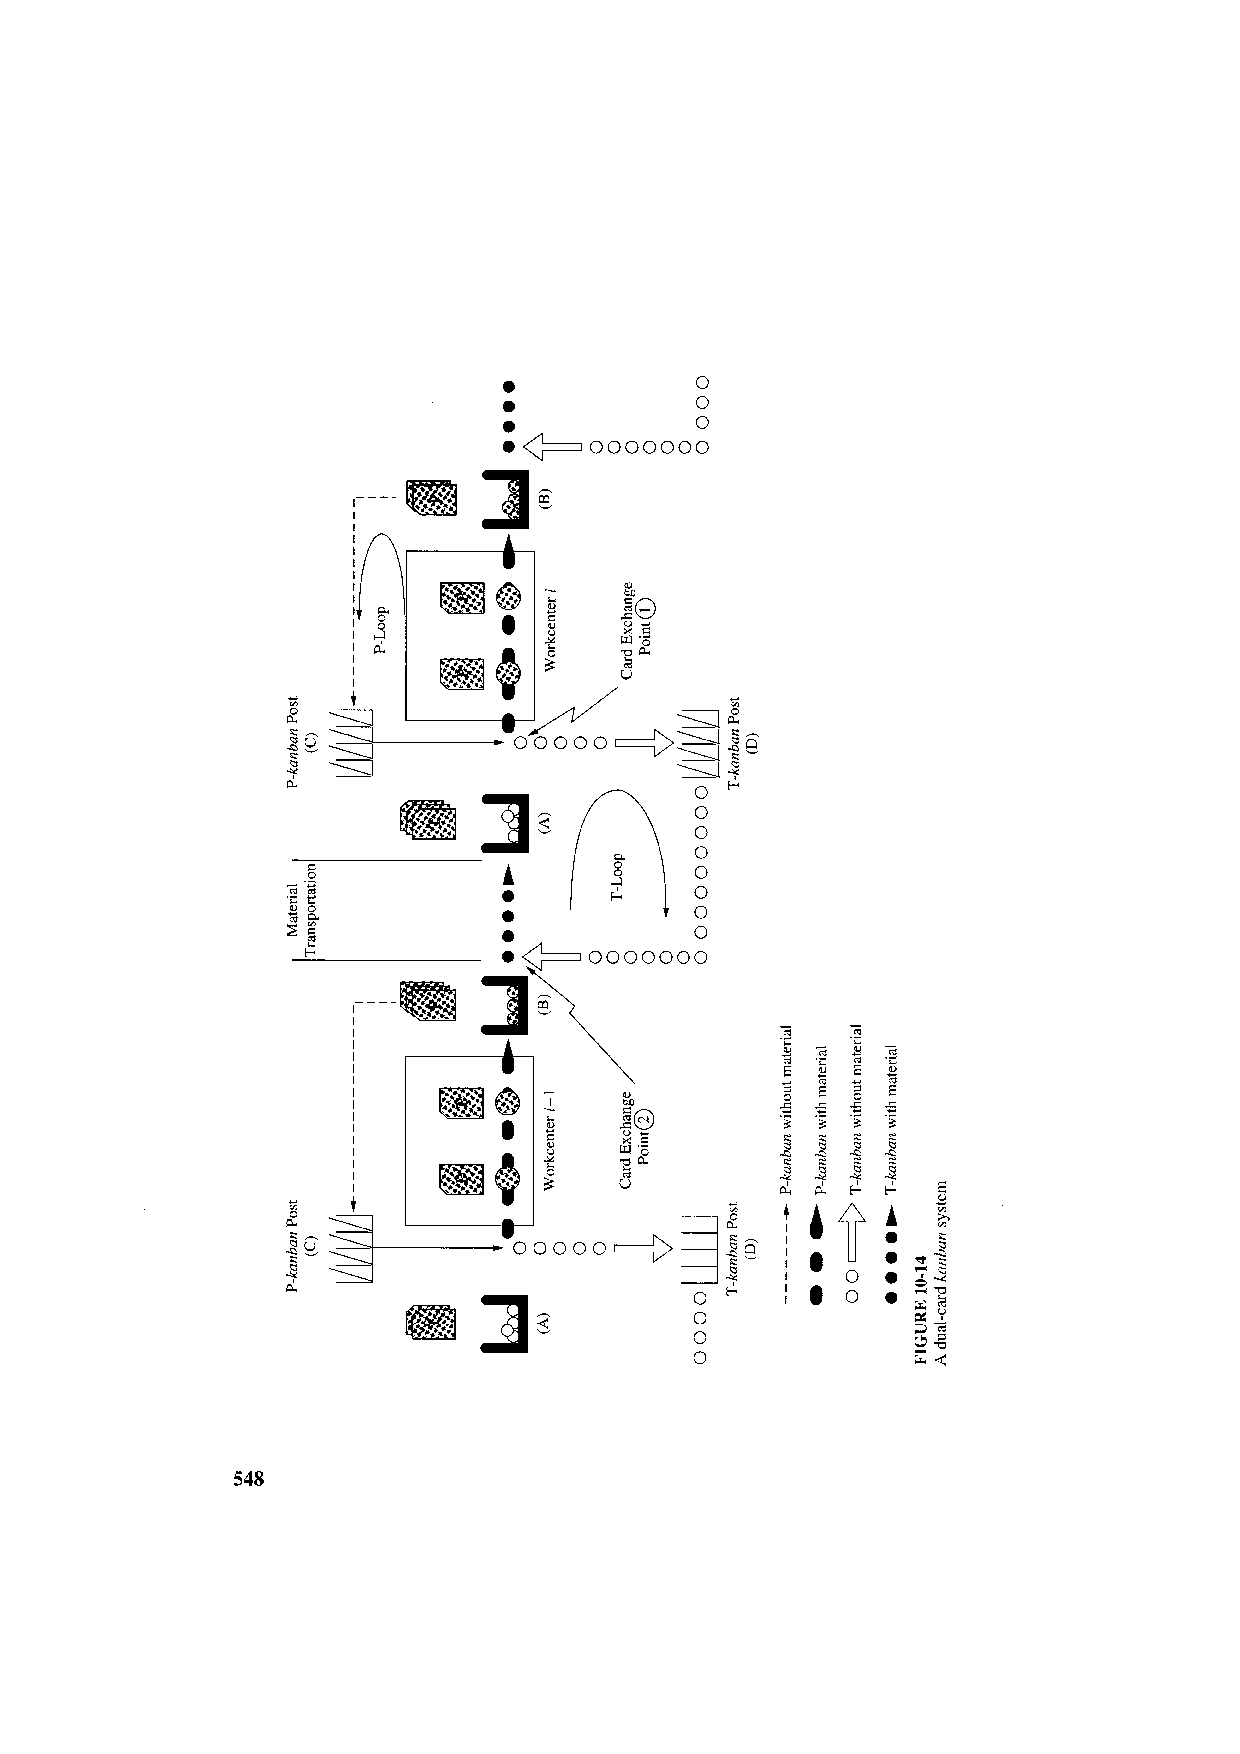
\includegraphics[angle=270,scale = 0.64,trim=20mm 30mm 30mm 30mm]{Figure10-14.pdf}}
\end{center}
We see an input store (A), output store (B), P-kanban posts (C) and T-kanban posts (D).\\
Parts are stored in containers. Each container holds a fixed amount of product that a P-kanban authorizes to produce, or a T-kanban authorizes to move. Each container in the input store has a T-kanban attached. Similarly, each container in the output store (B) has a P-kanban attached.\\
\textbf{P-loop} When a number of P-kanbans is accumulated at the P-kanban post (C) of workcenter $i$, it signals workcenter $i$ to produce a batch.  P-kanbans are removed from the post to the card exchange point (1) at the input store (A). There, the T-kanban is removed from each container and replaced by a P-kanban. The T-kanbans are placed in the T-kanban post (D). The number of containers in this exchange is equal to the number of P-kanbans on the post. Production starts and each container has its P-kanban attached. Upon completition, the finished batch is placed in output store (B) with the P-cards still attached. When a container is removed from the output store (B), its P-kanban is detached and again placed on the P-kanban post (C). The P-kanban post makes the kanbans visible and shows the queue of work to be performed in the cell.\\*
\textbf{T-loop} The exact same strategy is used for the T-kanbans.
\paragraph{Single-Card Systems} No P-kanbans.\\
Push/schedule-driven production $\rightarrow$ Inventory will be higher.
\setcounter{subsubsection}{4}
\subsubsection{JIT Models}
\paragraph{Sequencing Mixed-Model Pull Production Systems}\mbox{}\\
$n$: the number of different products to be made\\*
$D_i$: the integral number of units demanded over the scheduling horizon for product $i$\\*
$T = D_1 + D_2 + \dots + D_n$: the total number of units of all products made, also the time 'in units' to produce all items\\
The ideal production rate for product $i$ at time $t$ is given by
\begin{center}
$tD_i/\sum_{k=1}^tD_k$
\end{center}
Solving this scheduling problem is difficult. On the contrary, the next approach is useful:\\*
$j$ is the index for each unit of product $i$ (goes from $1$ to $D_{i}$)\\*
$d_{ij}$ is the ideal due date\\
$d_{i1} = T/(2D_i)$\\*
$d_{i2} = d_{i1} + T/D_{i}$\\*
$d_{ij} = (j - 1/2)T/D_i$\\
Assume $T = 10$ and $D_1 = 2$, then $d_{11} = 2.5$, $d_{12} = 7.5, d_{13} = 12.5$, \dots
\paragraph{Number of Kanbans Required}\mbox{}\\
$n$: number of P-and T-kanban sets for a given part\\*
$D$: demand per unit time, usually a day\\*
$L$: average lead time for the kanban\\*
$t_p$: average processing time per container\\*
$t_w$: average waiting during the production process plus transportation time per container\\*
$C$: container capacity, in units of products (not more than $10\%$ of daily demand)\\*
$\alpha$: a safety coefficient (not over $10\%$) - burgie style!\\*
then
\begin{center}
$L = t_p + t_w$\\*
$n = \cfrac{DL(1+\alpha)}{C}$
\end{center}
\subsubsection{CONWIP Models}
CONWIP stands for CONstant Work In Progress. Like kanban, CONWIP relies on an information signal. The card is attached to a container at the beginning of the line and travels with it until the end of the line. At that point, the card is removed from the container and returned to a card queue at the beginning of the line. So, the card traverses a circuit that includes the whole production line.
\paragraph{Controlling CONWIP-Based Production}\mbox{}\\
$n$: the card or container count\\*
$Flowtime = \cfrac{WIP}{Input rate}$\\*
The input rate is obviously the same as the output rate. We assume
\begin{itemize}
\item Infinite demand, which implies maximum level of WIP, and the line is working all the time.
\item Processing times are fixed. This is a reasonable assumption, since in a highly automated production environment, process variability is very small.
\item A single item is being produced.
\end{itemize}
Let
\begin{center}
$m$: number of machines\\*
$n$: the container count\\*
$t_i$: processing time on machine $i$\\*
$t_{BN}$: processing time on the bottleneck machine
\end{center}
Queues can only occur before the bottleneck machine. The time it takes to return to the bottleneck is the sum of the processing times on all other nonbottleneck machines.
\begin{center}
$\sum_{i = 1}^{m}t_i - t_{BN}$
\end{center}
During this time, the bottleneck must process all other $(n-1)$ containers.
\begin{center}
$(n-1)t_{BN}$
\end{center}
The time it takes for a container to reach the bottleneck must be less than or equal to the time it takes for the bottleneck to process all other $n-1$ containers.
\begin{center}
$(n-1)t_{BN} \ge \sum_{i=1}^{m}t_i - t_{BN}$
\end{center}
So
\begin{center}
$n = \sum_{i=1}^{m}t_i/t_{BN}$
\end{center}
Of course, we could easily come to this formula by just thinking, without the previous bullshit.
\paragraph{Evaluating Performance of CONWIP Control}\mbox{}\\
$i$: index of workstations\\*
$l$: number of containers\\*
$W(l)$: system relative throughput as a function of the number of containers $l$\\*
$N_i(l)$: number of containers at workstation $i$ as a function of the number of containers $l$\\*
$F_i(l)$: flowtime at workstation $i$ as a function of the number of containers $l$\\*
$\mu_i$: average processing rate at workstation $i$\\
$N_i(l)$ and $F_i(l)$ are random variables. Therefore, computations are performed on expected values. Execute the next algorithm:
\begin{itemize}
\item Set $E[N_i(0)] = 0$ for all $i = 0 \dots m$
\item For $l = 1, \dots, n$ calculate
\begin{center}
$E[F_i(l)] = \cfrac{E[N_i(l-1) + 1]}{\mu_i}$ $i = 1, \dots, m$\\*
$W(l) = \cfrac{l}{\sum_{i=0}^{m}E[F_i(l)]}$\\*
$E[N_i(l)] = W(l)E[F_i(l)]$ $i = 1, \dots, m$
\end{center}
\item Stop.
\end{itemize}
See Appendix \ref{sec:EvalutationofCONWIPControl} for a full example.
\clearpage
\begin{appendices}
\section{Example 4-3. Double exponential smoothing}
\label{sec:DoubleExponentialSmoothingExample}
\begin{center}
\fbox{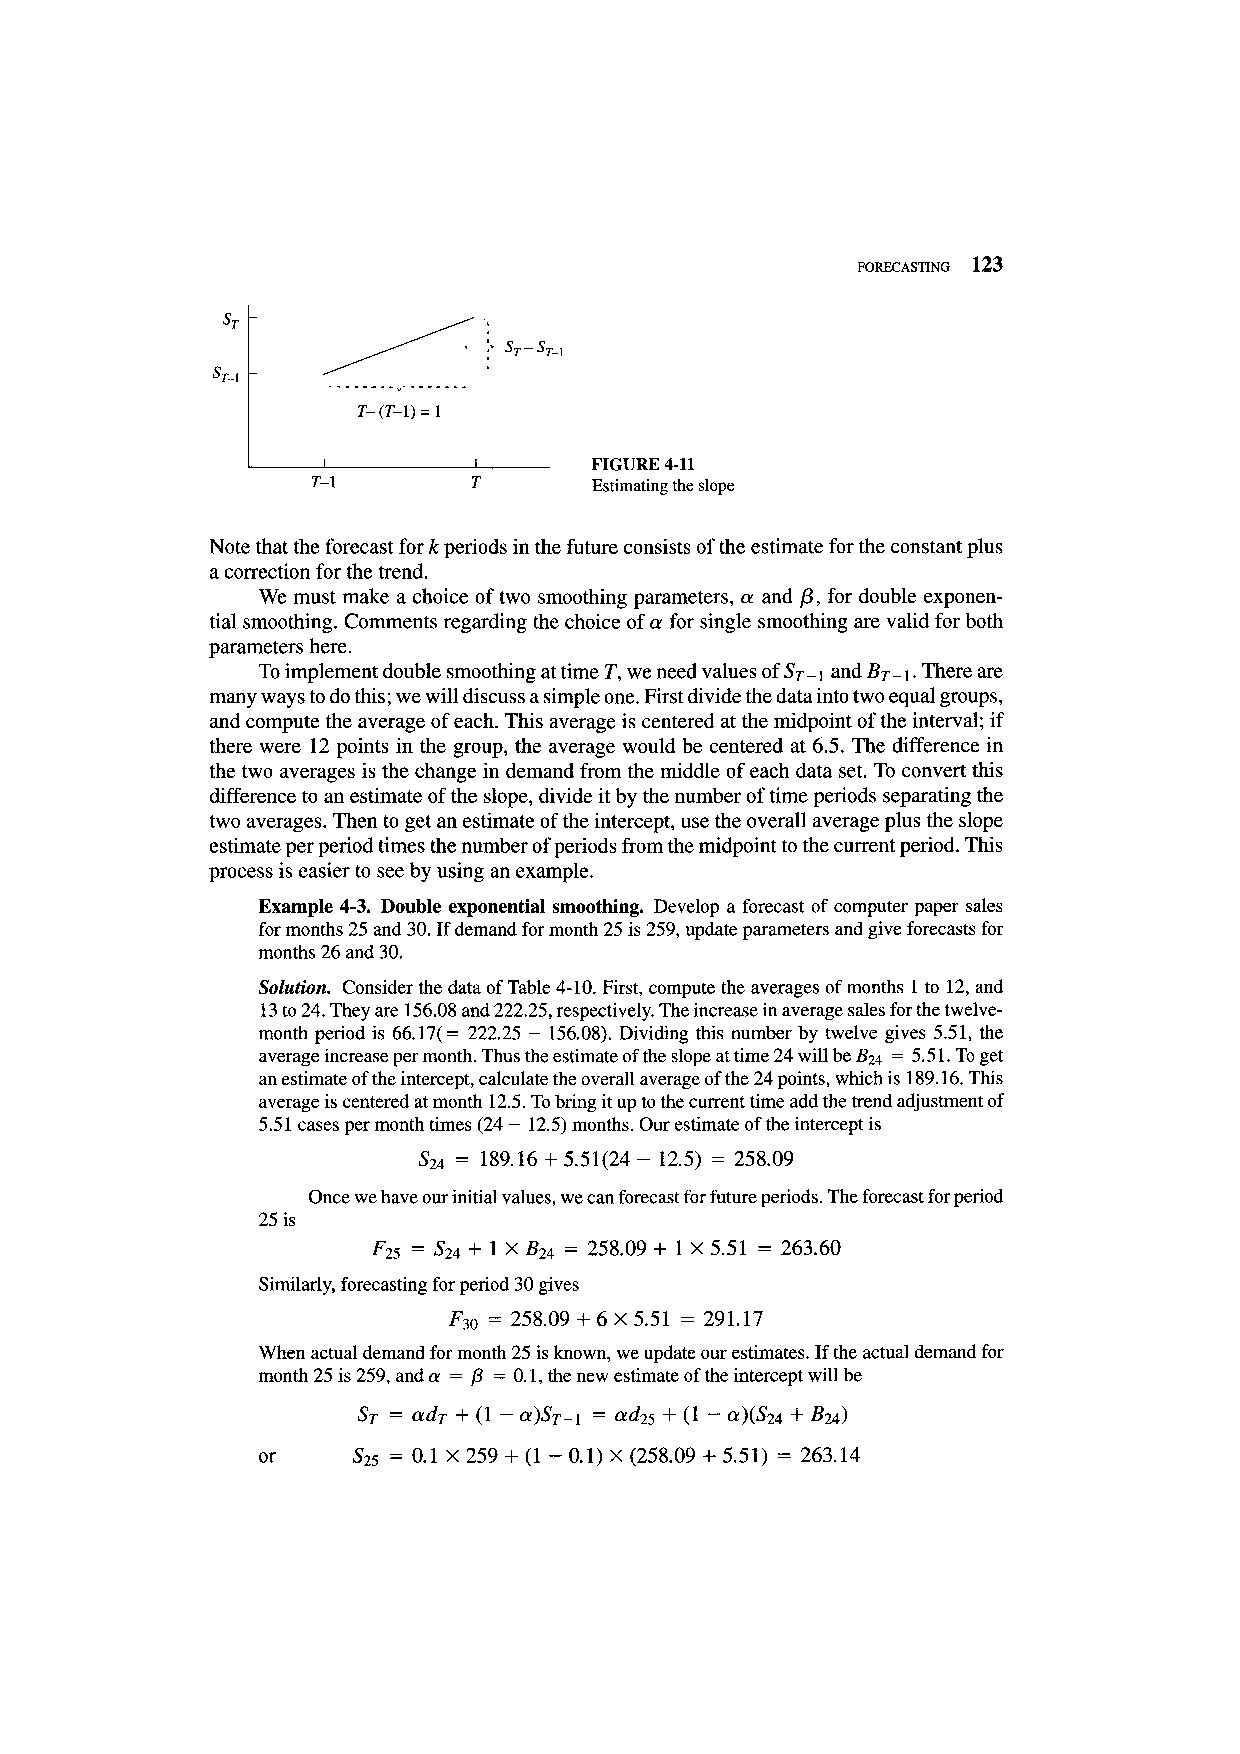
\includegraphics[scale = 0.85,trim=10mm 30mm 10mm 30mm]{Example4-3-page1.pdf}}
\end{center}
\begin{center}
\fbox{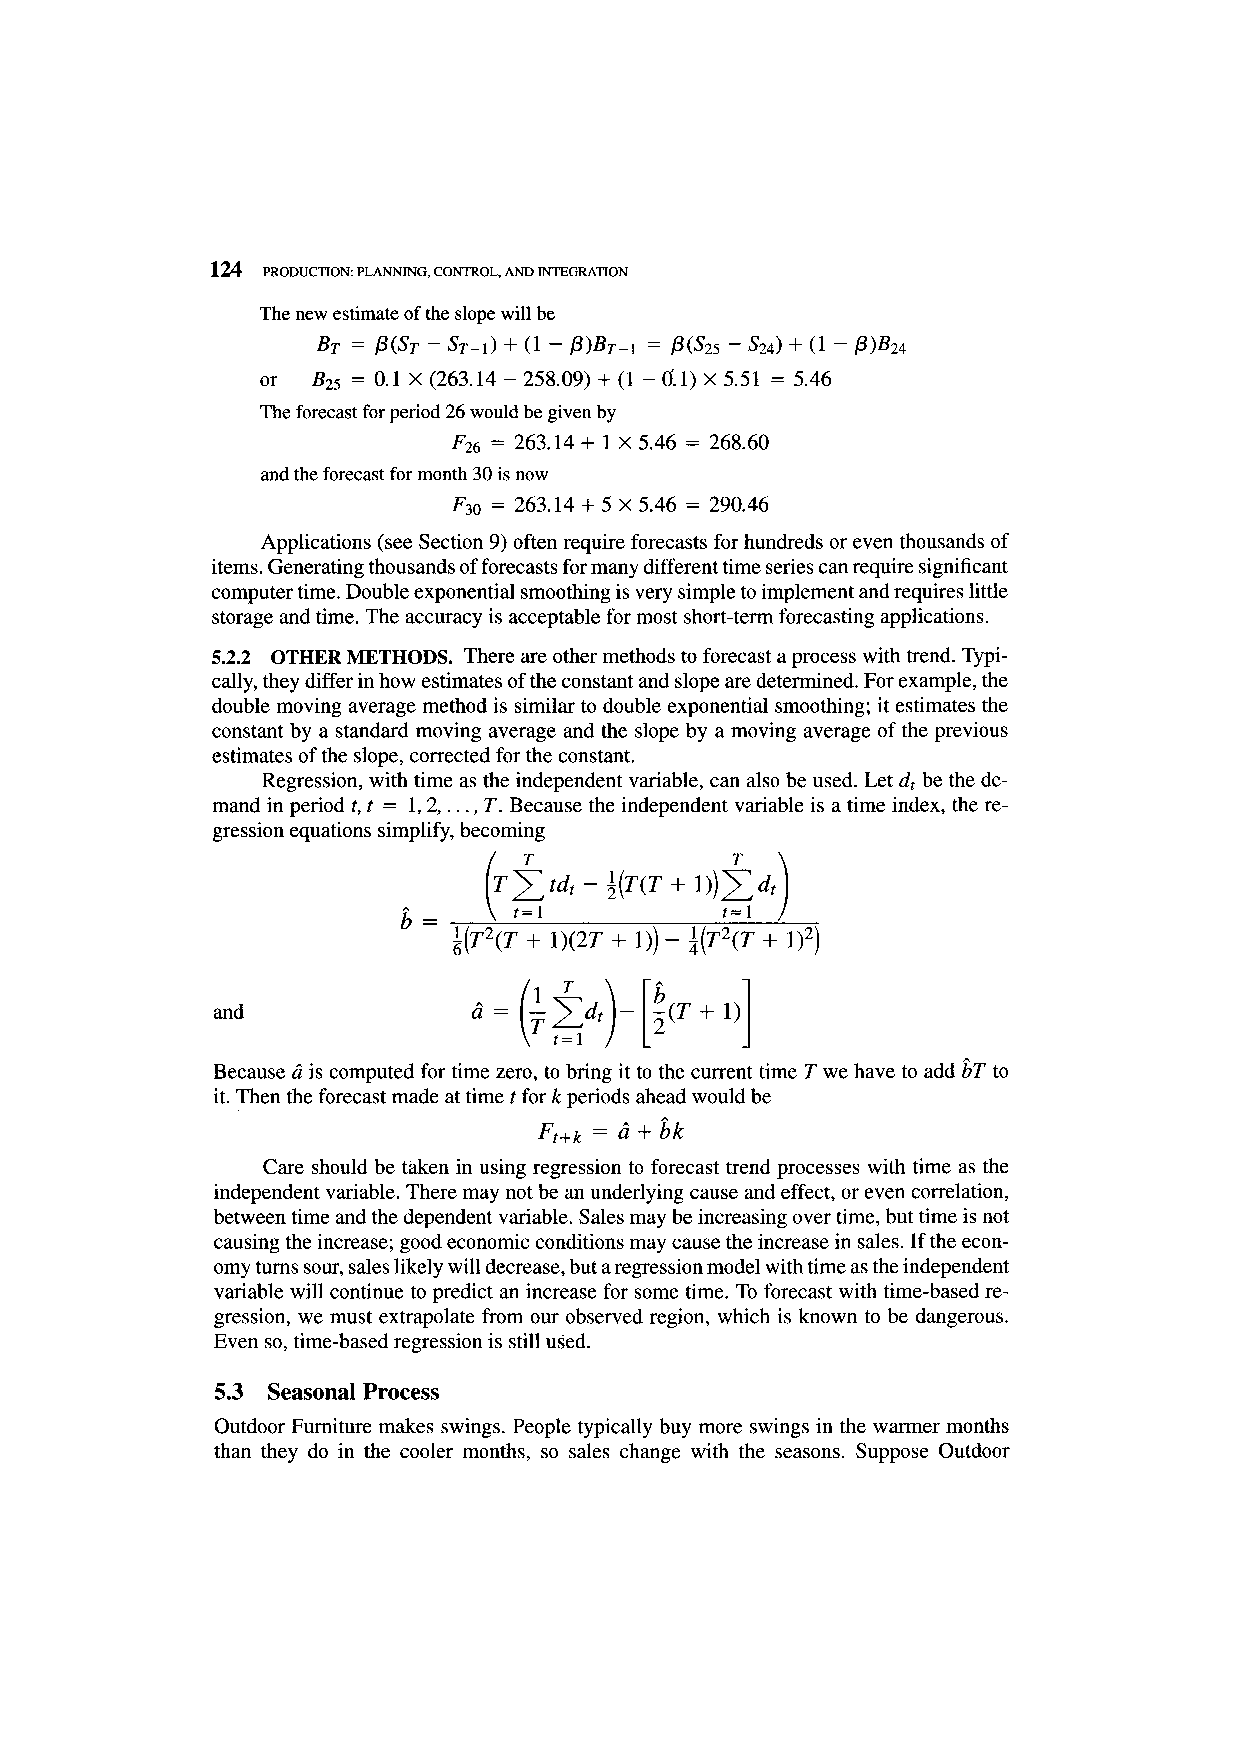
\includegraphics[scale = 0.85,trim=10mm 30mm 10mm 30mm]{Example4-3-page2.pdf}}
\end{center}
\section{Example 10-3. Evaluation of CONWIP Control}
\label{sec:EvalutationofCONWIPControl}
\begin{center}
\fbox{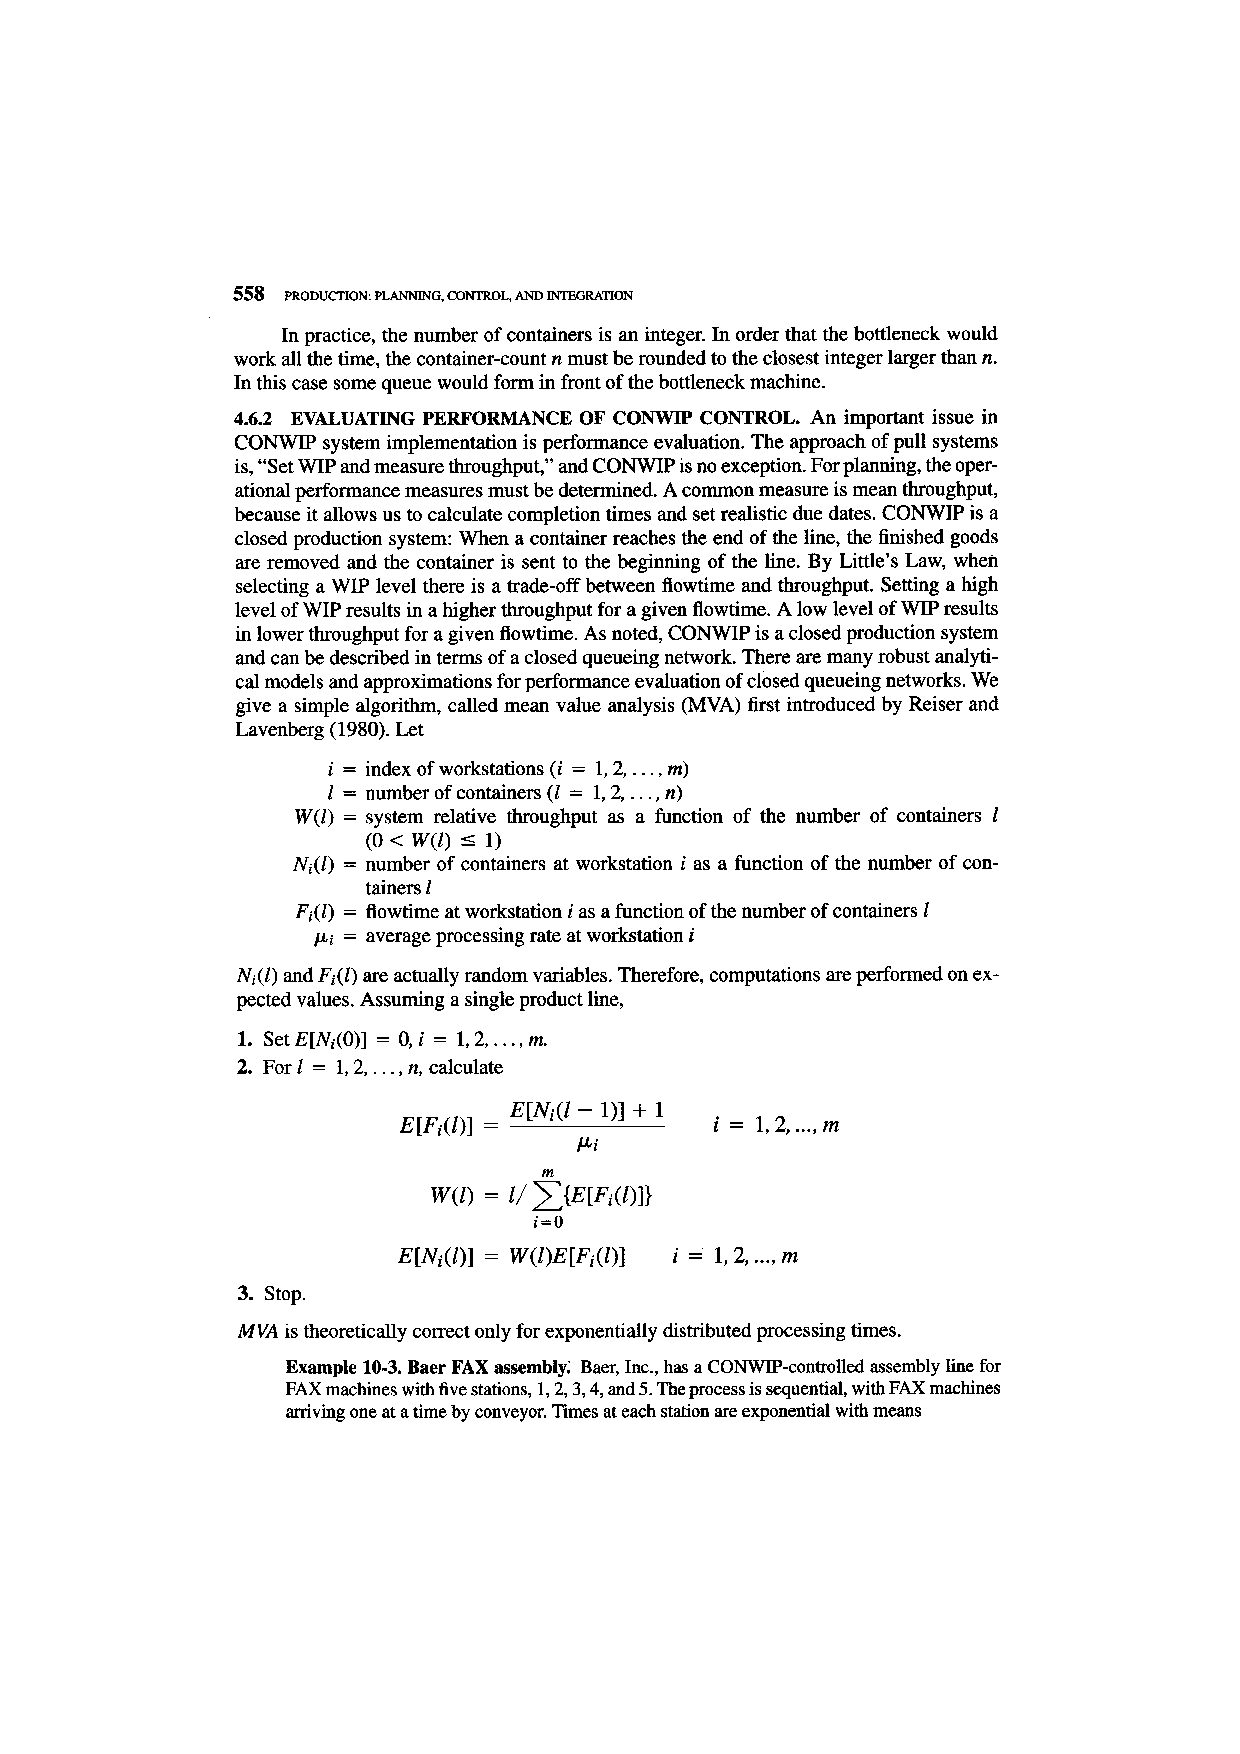
\includegraphics[scale = 0.85,trim=10mm 30mm 10mm 30mm]{Example10-3-page1.pdf}}
\end{center}
\begin{center}
\fbox{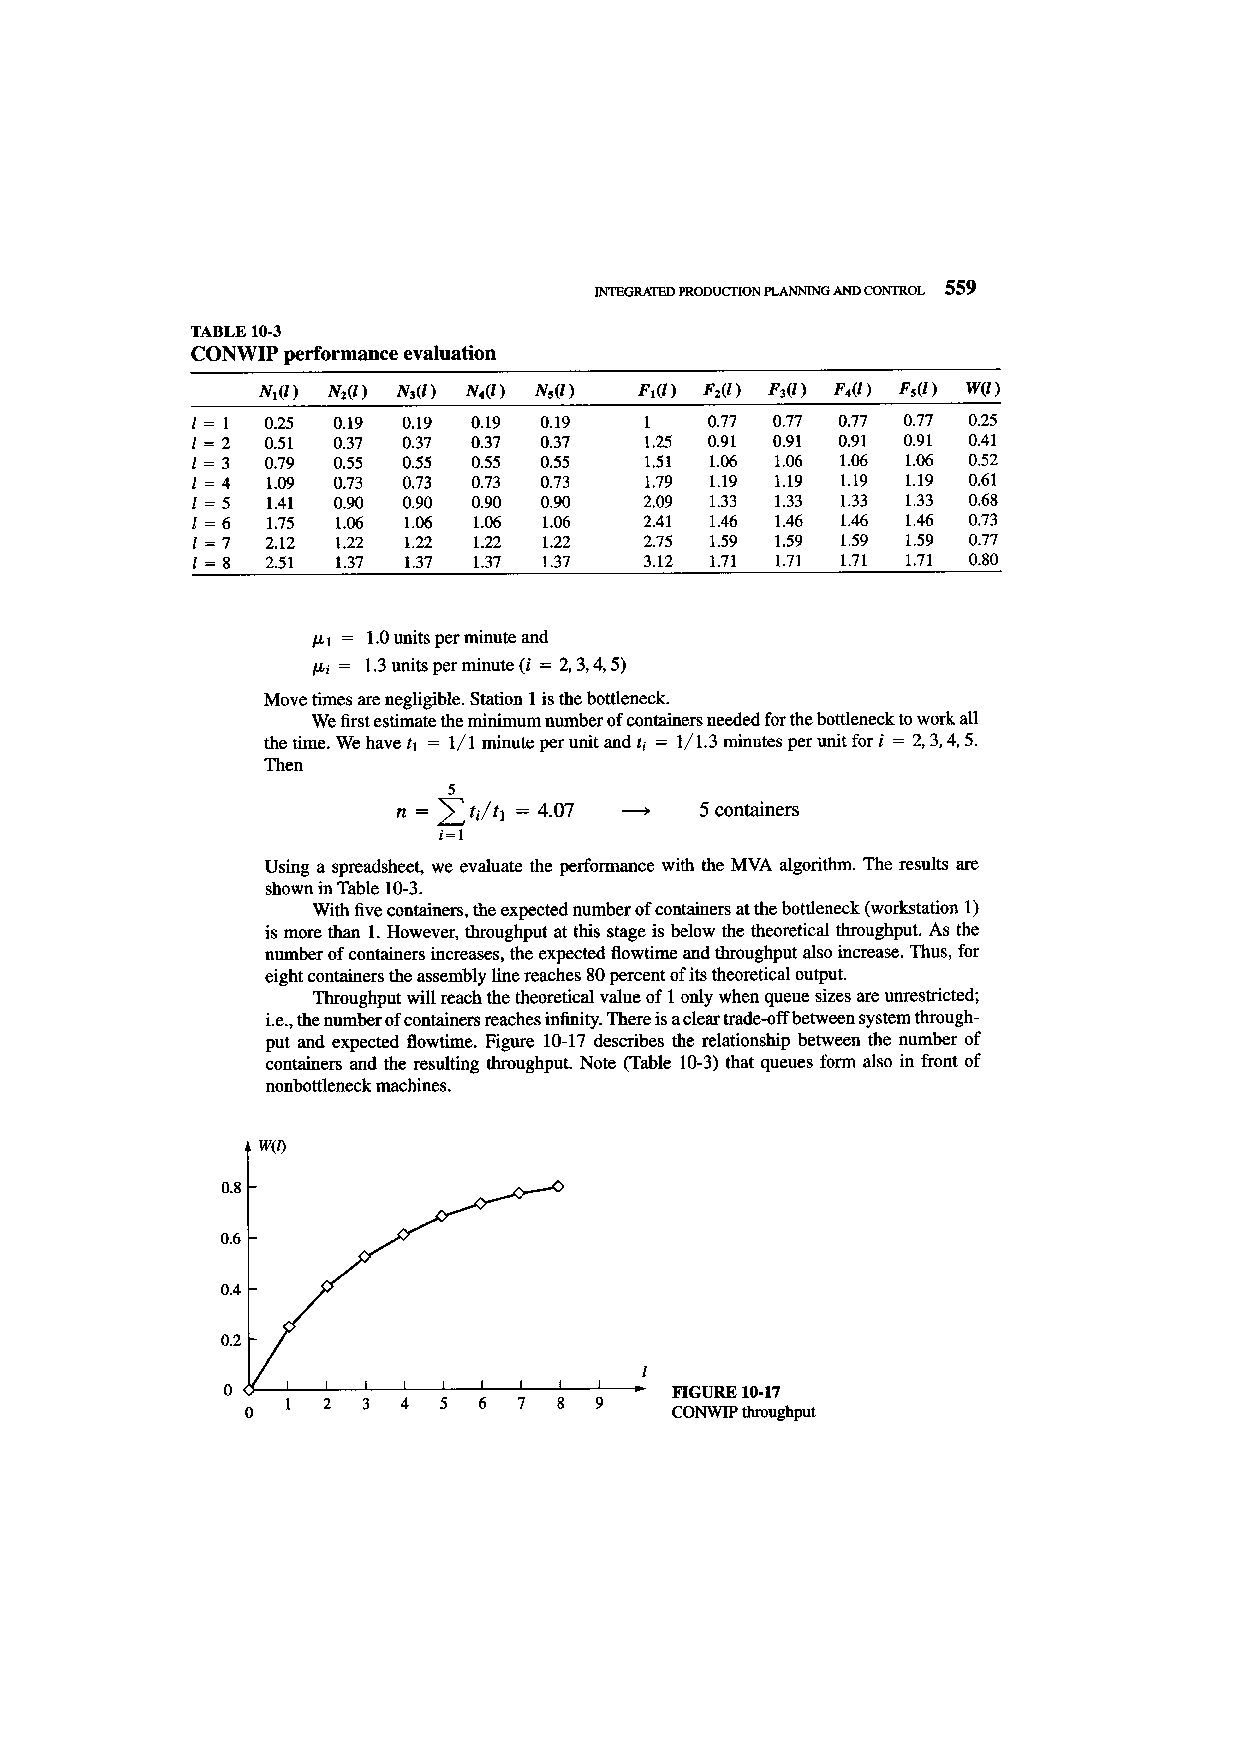
\includegraphics[scale = 0.85,trim=10mm 30mm 10mm 30mm]{Example10-3-page2.pdf}}
\end{center}
\section{Begrippenlijst}
\label{sec:Begrippen}
\begin{center}
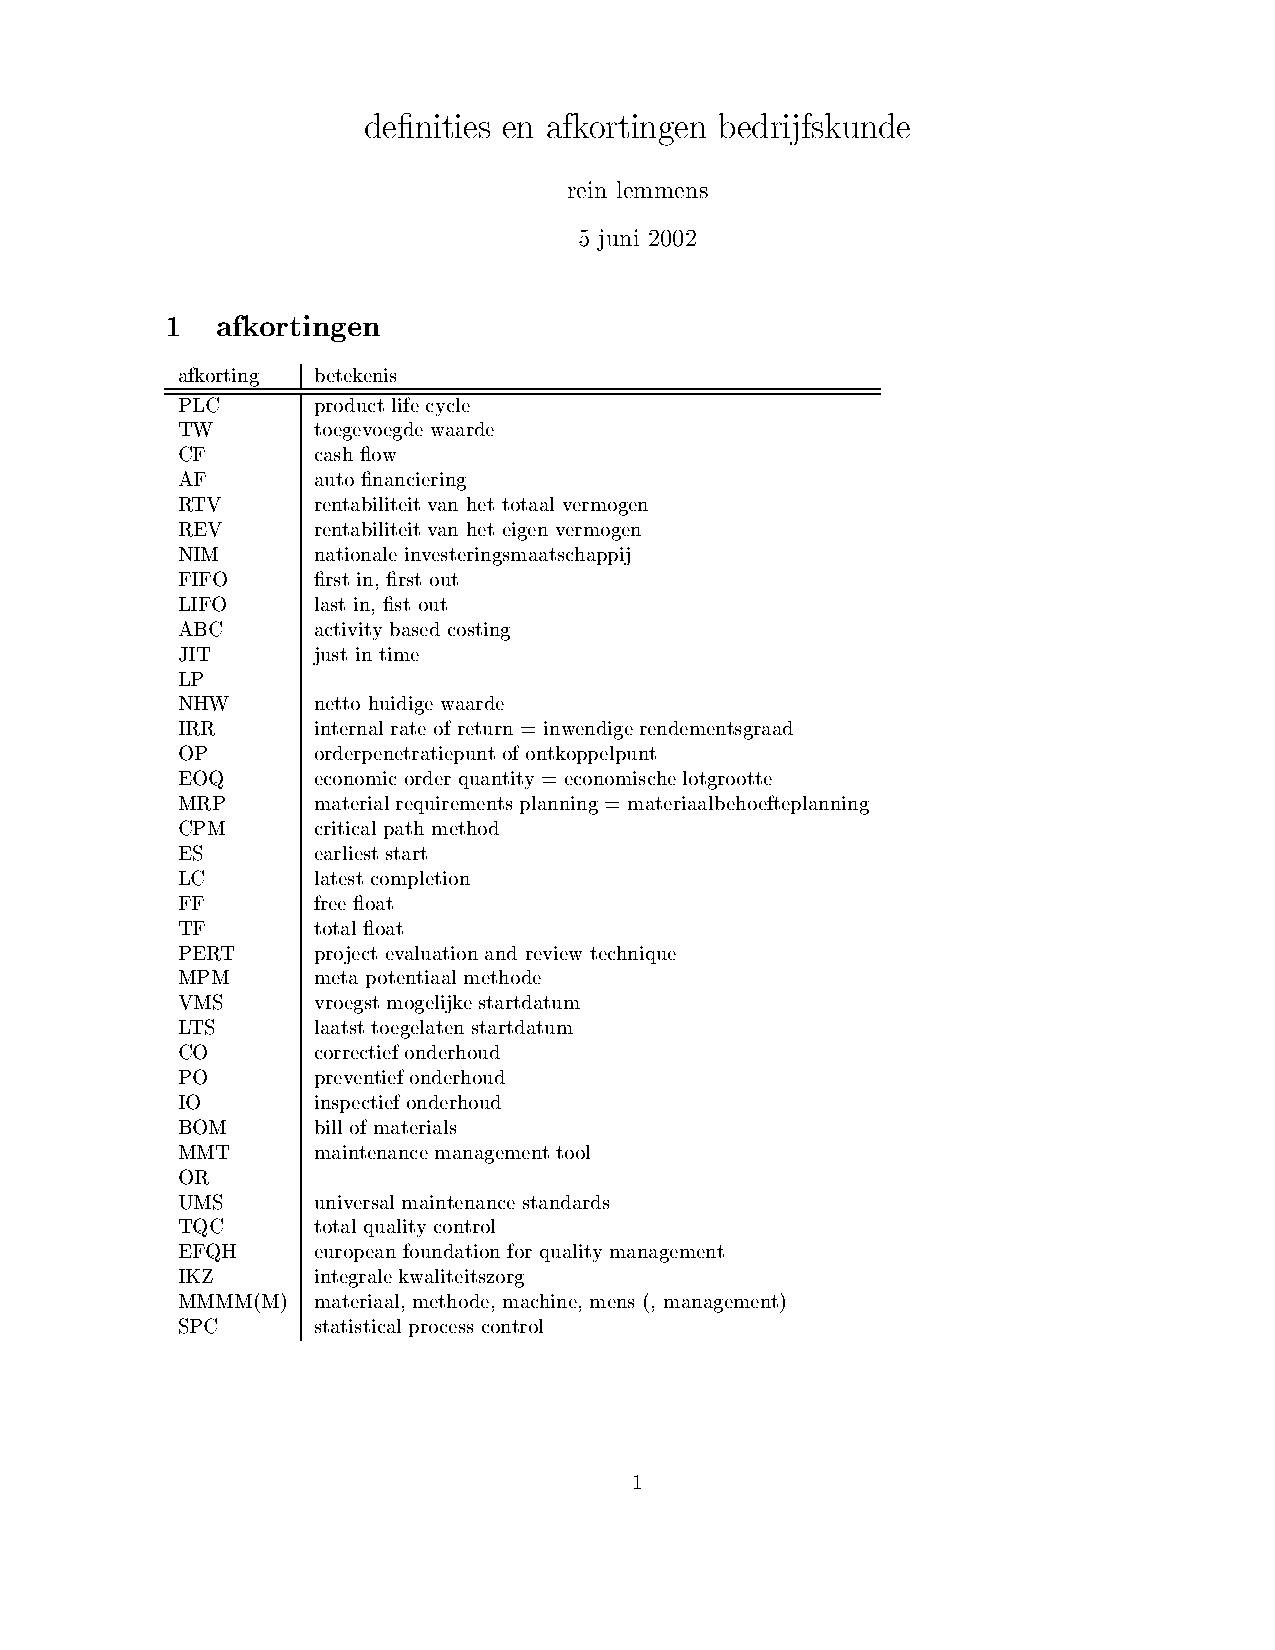
\includepdf[pages=-]{Begrippen.pdf}
\end{center}
\end{appendices}
\end{document}
